%%
%% Automatically generated file from Doconce source
%% (https://github.com/hplgit/doconce/)
%%
% #ifdef PTEX2TEX_EXPLANATION
%%
%% The file follows the ptex2tex extended LaTeX format, see
%% ptex2tex: http://code.google.com/p/ptex2tex/
%%
%% Run
%%      ptex2tex myfile
%% or
%%      doconce ptex2tex myfile
%%
%% to turn myfile.p.tex into an ordinary LaTeX file myfile.tex.
%% (The ptex2tex program: http://code.google.com/p/ptex2tex)
%% Many preprocess options can be added to ptex2tex or doconce ptex2tex
%%
%%      ptex2tex -DMINTED myfile
%%      doconce ptex2tex myfile envir=minted
%%
%% ptex2tex will typeset code environments according to a global or local
%% .ptex2tex.cfg configure file. doconce ptex2tex will typeset code
%% according to options on the command line (just type doconce ptex2tex to
%% see examples). If doconce ptex2tex has envir=minted, it enables the
%% minted style without needing -DMINTED.
% #endif

% #define PREAMBLE

% #ifdef PREAMBLE
%-------------------- begin preamble ----------------------

\documentclass[%
twoside,                 % oneside: electronic viewing, twoside: printing
final,                   % or draft (marks overfull hboxes, figures with paths)
10pt]{article}

\listfiles               % print all files needed to compile this document

\usepackage{relsize,epsfig,makeidx,color,setspace,amsmath,amsfonts}
\usepackage[table]{xcolor}
\usepackage{bm,microtype}

\usepackage{ptex2tex}

% #ifdef MINTED
\usepackage{minted}
\usemintedstyle{default}
% #endif

\usepackage[T1]{fontenc}
%\usepackage[latin1]{inputenc}
\usepackage[utf8]{inputenc}

\usepackage{lmodern}         % Latin Modern fonts derived from Computer Modern

% Hyperlinks in PDF:
\definecolor{linkcolor}{rgb}{0,0,0.4}
\usepackage[%
    colorlinks=true,
    linkcolor=linkcolor,
    urlcolor=linkcolor,
    citecolor=black,
    filecolor=black,
    %filecolor=blue,
    pdfmenubar=true,
    pdftoolbar=true,
    bookmarksdepth=3   % Uncomment (and tweak) for PDF bookmarks with more levels than the TOC
            ]{hyperref}
%\hyperbaseurl{}   % hyperlinks are relative to this root

\setcounter{tocdepth}{2}  % number chapter, section, subsection

% Tricks for having figures close to where they are defined:
% 1. define less restrictive rules for where to put figures
\setcounter{topnumber}{2}
\setcounter{bottomnumber}{2}
\setcounter{totalnumber}{4}
\renewcommand{\topfraction}{0.85}
\renewcommand{\bottomfraction}{0.85}
\renewcommand{\textfraction}{0.15}
\renewcommand{\floatpagefraction}{0.7}
% 2. ensure all figures are flushed before next section
\usepackage[section]{placeins}
% 3. enable begin{figure}[H] (often leads to ugly pagebreaks)
%\usepackage{float}\restylefloat{figure}

% prevent orhpans and widows
\clubpenalty = 10000
\widowpenalty = 10000

% --- end of standard preamble for documents ---


% insert custom LaTeX commands...

\raggedbottom
\makeindex

%-------------------- end preamble ----------------------

\begin{document}

% #endif


% ------------------- main content ----------------------



% ----------------- title -------------------------

\thispagestyle{empty}

\begin{center}
{\LARGE\bf
\begin{spacing}{1.25}
Geographic models 
\end{spacing}
}
\end{center}

% ----------------- author(s) -------------------------

\begin{center}
{\bf Torbjørn Seland${}^{}$} \\ [0mm]
\end{center}

    \begin{center}
% List of all institutions:
\end{center}

% ----------------- end author(s) -------------------------

\begin{center}
Nov 25, 2014
\end{center}

\vspace{1cm}


\tableofcontents


\vspace{1cm} % after toc




\section{Introduction}
This chapter will introduce a new model for epidemic diseases. By expand the ODE system from previous chapter to also consist a term for geographic spread of. The first section \emph{Simple system for spatial spread} will build on the simple SIR model presented in previous chapter and be based on \emph{Geographic spread and Control of epidemics} by Murray \cite{murray2003mathematical}. The parameters from \emph{English Boarding School} in previous chaper will be used for the model and the result will be compared between the models. The position of the infected student will be compared against the number of infected each day. The last section,*Zombiefication*, will study and expand the system from Langtangen, Mardal and Røtnes \cite{zombie-math}. The results and parameter values used to calculate \emph{Walking Dead} will be used to simulate the geographic result.


\section{Simple system for spatial spread}
A spatial variable, \textbf{x} will now be introduced to the model. This result in both temporal and spatial variations. The difference from a standard ODE system will be the diffusion part added to each equation. The system can be seen in eq(\ref{eq:simple_PDE}). 
\begin{equation} \label{eq:simple_PDE}
	\begin{aligned}
	\frac{\partial S}{\partial t} &= -rIS + D\nabla ^2 S\\
	\frac{\partial I}{\partial t} &= rIS- aI + D\nabla ^2 I\\
	\frac{\partial R}{\partial t} &= aI + D\nabla ^2 R
	\end{aligned}
\end{equation}
With the following conditions for the boundary and initial values
\begin{equation} \label{eq:boundary_initial}
	\begin{aligned}
	u_x(0,t) &= u_x(X,t) = 0,\quad u = S,I,R\\
	u(x,0) &= f_u(x),\quad u= S,I,R
	\end{aligned}
\end{equation}
This result in Neumann conditions at the boundary. The following implementation can be used at the boundary
\begin{equation}
	\begin{aligned}
	\frac{u_{-1}^n - u_1^n}{2\Delta x} &= 0
	u_{-1}^n &= u_1^n
	\end{aligned}
\end{equation}
This is solved by adding an extra point on each side, called ghost points. The values in these points are updated each time step with values from $u_1^n$ and $u_{X-1}^n$ each round. All three classes, $S,I,R$ have the same diffusion coefficient, $D$, for this system. This give the three groups the same diffusion speed. This can vary between systems. Section \emph{Zombiefication}, will contain various diffusion constants. The two parts $rIS$ and $aI$ will work in the same way as in the ODE system. Since this model taking the position into account, the idea is to model a group of infective that moves into a uniform population with susceptible, which is spread around with the density $S_0$. Then the geotemporal spread can be seen. The problem will first be consider as one-dimensional. The system can be nondimensionalise by writing 
\begin{equation} \label{eq:constants_nondimensional}
	\begin{aligned}
	I^* =\frac{I}{S_0},&\quad I^* = \frac{I}{S_0},&\quad R^*= \frac{R}{S_0},&\\
	x^* =\left(\frac{rS_0}{D}\right)^{1/2}x,&\quad t^*=rS_0t,&\quad \lambda =\frac{a}{rS_0},&
	\end{aligned}
\end{equation}
$S_0$ is used as a representative population. Now the model(\ref{eq:simple_PDE}) can be expressed as in eq(\ref{eq:simple_non_PDE}). The asterisks have been dropped to make it easier to read.
\begin{equation} \label{eq:simple_non_PDE}
	\begin{aligned}
	\frac{\partial S}{\partial t} &= -IS + \frac{\partial^2 S}{\partial x^2},\\
	\frac{\partial I}{\partial t} &= IS- \lambda I + \frac{\partial^2 I}{\partial x^2},\\
	\frac{\partial R}{\partial t} &= \lambda I + \frac{\partial^2 R}{\partial x^2},
	\end{aligned}
\end{equation}
The three parameters $r$, $a$ and $D$ have been replaced by $\lambda$. The \emph{reproduction rate} that was presented for the ODE model can be seen as $1/\lambda $. This has a couple of equivalent meanings. $1/\lambda$ can be seen as the number of secondary infections produced by one primary infected. It can also be used to measure two different time scales. The first one, $1/(rS_0)$, measure the contagious time of the disease. The second one can look at the life expectancy for an infective. This can be described $1/a$. 
\subsection{Travelling wave 1D}
This section will focus on the travelling wave. The travelling wave describe how a group of infected, in this case, travels through a geographic area of humans. This will be shown by sending a pulse of infected into a group of susceptible. A travelling wave solution will be described as follows,
\begin{equation} \label{eq:trav_para}
I(x,t)=I(z),\quad S(x,t)=S(z),\quad R(x,t) = R(z),\quad z = x-ct,
\end{equation}
The value $c$ describe the wave speed. This represents a wave of constant shape that travels in the positive x-direction. (\ref{eq:trav_para}) can be inserted into (\ref{eq:simple_non_PDE}). This result in the ordinary system(\ref{eq:ord_diff_sys})
\begin{equation} \label{eq:ord_diff_sys}
	\begin{aligned}
	S'' + cS' - IS &= 0,\\
	I'' + cI' + I(S-\lambda)&=0\\
	R'' + cR  + I\lambda &=0
	\end{aligned}
\end{equation}
This gives an eigenvalue problem. The value of $\lambda$ needs to stay in a range where $c > 0$ is fulfilled. The values $S$, $I$ and $R$ have to stay nonnegative. This leads to
\begin{equation} 
	\begin{aligned}
	0 \leq S(-\infty) < S(\infty)&=1\\
	I(-\infty)=I(\infty)&=0,\\
	1 \geq R(-\infty)\geq R(\infty) &= 0
	\end{aligned}
\end{equation}

An epidemic wave can be seen in figure(\ref{fig:1D_sub}). The value of $\lambda$ is sat to 0.5. The initial value for \emph{Susceptible} is 1 for the area and the \emph{Removed} to 0. The \emph{Infected} class has a Gauss curve around 0 at initial time. In the four subplot, the epidemic wave travel towards the other side. The value $z$, which is defined in (\ref{eq:trav_para}), is used to plot the travelling wave measured at a specific point, in this case 15. This travelling wave is shown in figure(\ref{fig:1D_tw}).       


\begin{figure}[ht]
  \centerline{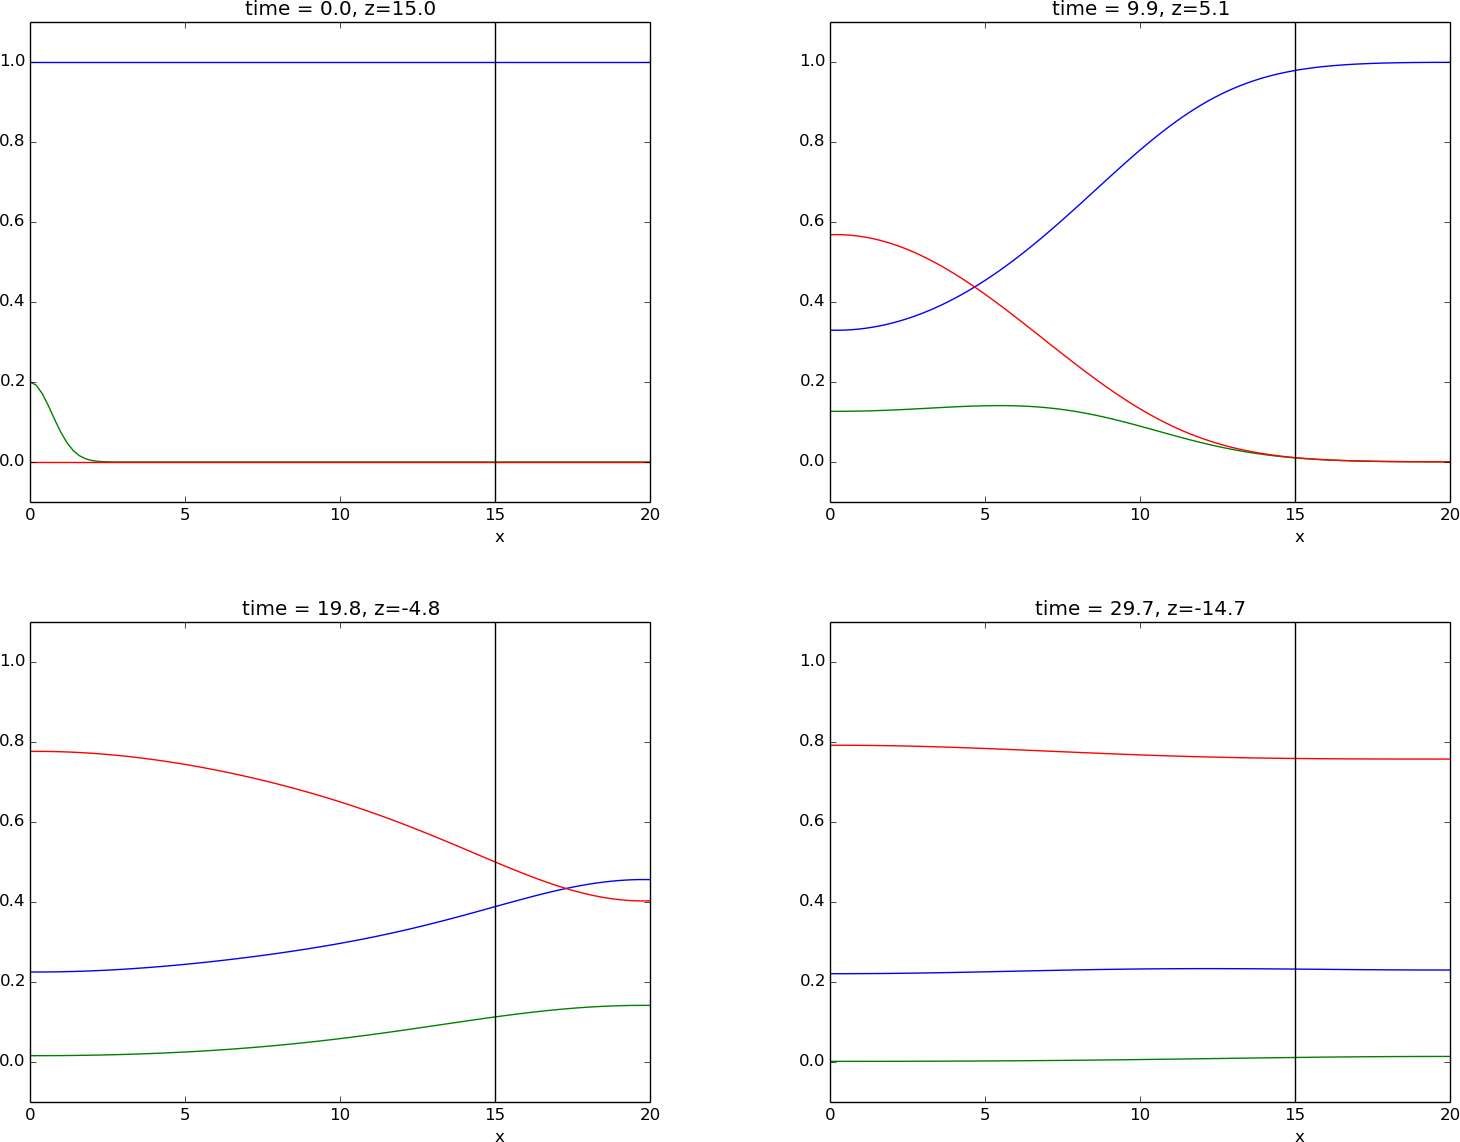
\includegraphics[width=0.8\linewidth]{plots/trav_wave_sub.eps}}
  \caption{
  \label{fig:1D_sub} The system (\ref{eq:ord_diff_sys}. A gaussian curve with height 0.2 placed on the left side. This causes an epidemic wave controlled by the parameter $\lambda=0.5$. The size is measured at point $x=15$ and can be seen in figure (\ref{fig:1D_tw}).
  }
\end{figure}
%\clearpage % flush figures fig:1D_sub



\begin{figure}[ht]
  \centerline{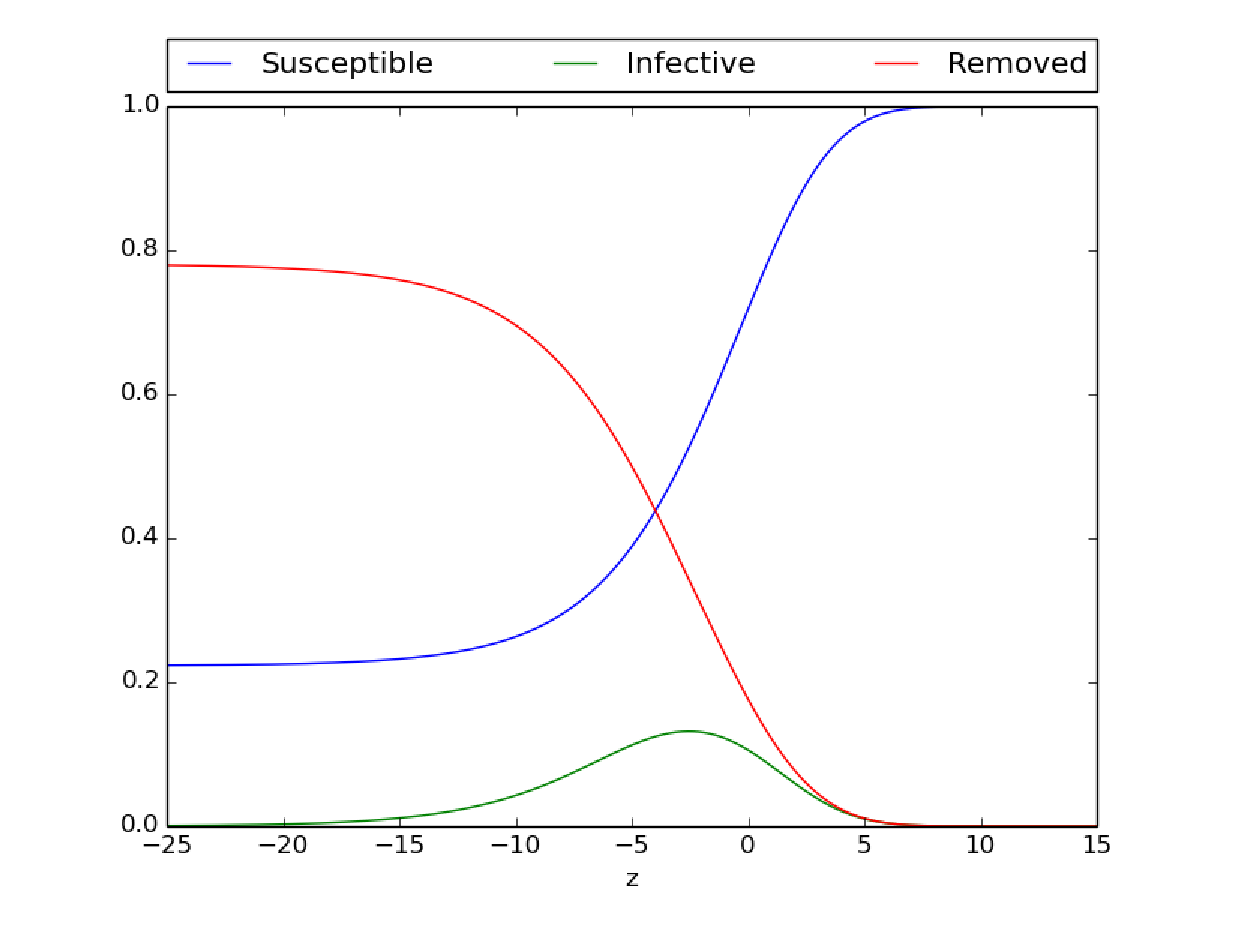
\includegraphics[width=0.9\linewidth]{plots/epidemic_wave_z_lambda_0_5.eps}}
  \caption{
  \label{fig:1D_tw} This shows the travelling wave measures at at $x=15$ in figure(\ref{fig:1D_sub})
  }
\end{figure}
%\clearpage % flush figures fig:1D_tw


The system(\ref{eq:ord_diff_sys}) is a fourth order phase space system. The lower bound for $c$ can be found. J.D Murray shows this in \cite{murray2003mathematical}. The \emph{Infective} class in system(\ref{eq:ord_diff_sys}) can be linearised when $z\rightarrow \infty$. This leads to $S\rightarrow 1$ and $I \rightarrow 0$. The result then become 
\begin{equation}
	I'' + cI' + I(S-\lambda) \approx 0 
\end{equation}
This can be found by
\begin{equation}
I(z) \varpropto \exp\left[(-c \pm {c^2 -4(1-\lambda)}^{1/2})z/2\right]
\end{equation}
Since a concentration cannot be negative, it is required that $I(z)\rightarrow 0$. Therefore the solution has to avoid oscillation around 0. If a travelling wave exist, it has to satisfy
\begin{equation}
	c \geq 2(1-\lambda)^{1/2}, \lambda < 1
\end{equation}
If $\lambda > 1$, no travelling wave will exist. Then the disease will die out. The terms defined in (\ref{eq:constants_nondimensional}) will give the threshold conditions,
\begin{equation}
	\lambda = \frac{a}{rS_0} < 1
\end{equation}
This is the same value that was given for the ODE model in the previous chapter.
\subsection{Verifying the solution}
To verify the implementation of the solution, a couple of tests can be done one the system. The system will be tested again a constant solution and a manufactured solution.   

\paragraph{Constant solution.}
A constant solution use preproduced constant values for for the concentrations $S$, $I$ and $R$. These can be replaced by $S = C_s,I=C_i,R=C_r$. The value of $C_i$ can only be 0 in system(\ref{eq:simple_non_PDE}). This results in a poor test where several bugs can escape. The system can be expanded by adding a term $\beta R$ to the \emph{Susceptible} class and subtract the same term from the \emph{Removed} class. Then all three values can be tested. The system will then look: 
\begin{equation} \label{eq:simple_non_PDE2}
	\begin{aligned}
	\frac{\partial S}{\partial t} &= -IS + \beta R + \frac{\partial^2 S}{\partial x^2},\\
	\frac{\partial I}{\partial t} &= IS- \lambda I + \frac{\partial^2 I}{\partial x^2},\\
	\frac{\partial R}{\partial t} &= \lambda I - \beta R + \frac{\partial^2 R}{\partial x^2},
	\end{aligned}
\end{equation}
By deriving (\ref{eq:simple_non_PDE2}), the following system (\ref{eq:constant_PDE}) has to be solved
\begin{equation} \label{eq:constant_PDE}
	\begin{aligned}
	C_iC_s &= \beta C_r \\
	C_iC_s &= \lambda C_i \\
	\lambda C_i &= -\beta C_r 
	\end{aligned}
\end{equation}

The values $\beta$ and $\lambda$ are based on the constants. These can be chosen freely. Here they are sat to $C_s = 1.2,C_i=0.8,C_r=0.6$. This result in $\lambda= C_s = 1.2$ and $\beta= \frac{C_s C_i}{C_r}=1.6$. A test is made in python and can be seen in the code.

\bpycod
def test_constant_solution():
    """
    Test problem where u=u_const is the exact solution, to be
    reproduced (to machine precision) by any relevant method.
    """
    def exact_solution(t):
        return C_s,C_i,C_r
    
    def lam(t,x):
        return C_s

    def beta(t,x):
        return (C_s*C_i)/float(C_r)

    #Constant values
    C_s = 1.2
    C_i = 0.8
    C_r = 0.6
    
    #lam = C_s
    #beta = (lam*C_i)/float(C_r)
    
    T = 2; Nt = 200
    X = 20; Nx = 40
    S_1 = np.ones(Nx+3)*C_s
    I_1 = np.ones(Nx+3)*C_i
    R_1 = np.ones(Nx+3)*C_r
    
    t,x,S,I,R = simple_PDE(T,Nx,Nt,X,lam,beta,S_1,I_1,R_1)
    
    S_e,I_e,R_e = exact_solution(t)
    difference = abs(S_e - S).max()  # max deviation
    tol = 1E-14
    assert difference < tol

    difference = abs(I_e - I).max()  # max deviation
    tol = 1E-14
    assert difference < tol

    difference = abs(R_e - R).max()  # max deviation
    tol = 1E-14
    assert difference < tol
\epycod

The test was run with no error, and the three constant values were produced correctly. This test is not good enough by it self to qualify the program, but an error here would result in a large error in the program that had to be fixed before the next test. 
\paragraph{Manufactured solution.}
By constructing a function to each equation in the system (\ref{eq:simple_non_PDE}), a manufactured solution can be created. Here $S$,$I$ and $R$ are pre produced. The system will be
\begin{equation} \label{eq:simple_non_PDE2}
	\begin{aligned}
	\frac{\partial S}{\partial t} &= -IS + \frac{\partial^2 S}{\partial x^2}+f(x,t),\\
	\frac{\partial I}{\partial t} &= IS- \lambda I + \frac{\partial^2 I}{\partial x^2}+g(x,t),\\
	\frac{\partial R}{\partial t} &= \lambda I + \frac{\partial^2 R}{\partial x^2}+h(x,t),
	\end{aligned}
\end{equation}
where $f$,$g$ and $h$ are functions to achieve the expected results for $S$, $I$ and $R$. In this case the functions will be:
\begin{equation}
	\begin{aligned}
	f(x,t) = \frac{\partial S}{\partial t} + IS - \frac{\partial^2 S}{\partial x^2}\\
	g(x,t) = \frac{\partial I}{\partial t} - IS + \lambda I - \frac{\partial^2 I}{\partial x^2}\\
	h(x,t) = \frac{\partial R}{\partial t} -\lambda I - \frac{\partial^2 R}{\partial x^2},
	\end{aligned}
\end{equation}
When choosing the expected function for the classes, it is important that the boundary conditions from (\ref{eq:boundary_initial}) is fulfilled.
\begin{equation}
    u_x(0,t) = u_x(X,t) = 0
\end{equation}
The quantities have been sat to:
\begin{equation}
	\begin{aligned}
    S(x,t) = cos(\frac{\pi}{X}x)t\\
    I(x,t) = cos(\frac{\pi}{X}x)t\\
    R(x,t) = cos(\frac{\pi}{X}x)t
	\end{aligned}
\end{equation}
Now \code{sympy} can be used to do the calculations for the three functions $f$, $g$ and $h$. The program can be seen in the Appendix. This result in the following equations seen in (\ref{eq:manu_func}) 

Which give
\begin{equation} \label{eq:manu_func}
	\begin{aligned}
	f(x,t) &= (t^2\cos(\pi x) + \pi^2t + 1)\cos(\pi x)\\
	g(x,t) &= (\lambda t - t^2\cos(\pi x) + \pi^2t + 1)\cos(\pi x)\\
	h(x,t) &= (-\lambda t + \pi^2t + 1)\cos(\pi x)
	\end{aligned}
\end{equation}
A similar test made for the constant solution can be used here. While the constant test expected a difference on machine precition, this is not the case here. In this test, an expected convergence rate can be measured.

The following manufactured test will then be
\bpycod
def test_manufactured_solution(T,Nt,X,Nx):
    """
    Test problem where u=c*t+I is the exact solution, to be
    reproduced (to machine precision) by any relevant method.
    """
    
    def exact_solution_S(t,x):
        return np.cos(np.pi*x)*t

    def exact_solution_I(t,x):
        return np.cos(np.pi*x)*t

    def exact_solution_R(t,x):
        return np.cos(np.pi*x)*t


    def beta(t,x):
        return exact_solution_S(t,x)*exact_solution_I(t,x)/exact_solution_R(t,x)
    lam = 1
    def f(t,x):
        return (t**2*np.cos(np.pi*x) + np.pi**2*t + 1)*np.cos(np.pi*x) 

    def g(t,x):
        return (lam*t - t**2*np.cos(np.pi*x) + np.pi**2*t + 1)*np.cos(np.pi*x)

    def h(t,x):
        return (-lam*t + np.pi**2*t + 1)*np.cos(np.pi*x)
        

    dx = X/float(Nx)
    dt = T/float(Nt)
    S_1 = exact_solution_S(0,np.linspace(0-dx,X+dx,Nx+3))
    I_1 = exact_solution_I(0,np.linspace(0-dx,X+dx,Nx+3))
    R_1 = exact_solution_R(0,np.linspace(0-dx,X+dx,Nx+3))
     
    t,x,S,I,R = simple_PDE(T,Nx,Nt,X,lam,beta,S_1,I_1,R_1,f,g,h)
    S_e = exact_solution_S(t[-1],x)
    I_e = exact_solution_I(t[-1],x)
    R_e = exact_solution_R(t[-1],x)
    
    difference_S = abs(S_e - S).max()  # max deviation

    
    #for i in range(4):
    #    print "n",i,"S_e",exact_solution_S(t[i],x)
    
    #print "S",S
    #t_tot = np.sum(t[:-1])
    #print "t_tot",t_tot
    #difference_exp = t_tot*dt*np.cos(x*np.pi)*((2*(np.cos(np.pi*dx)-1))/dx**2+np.pi**2)
    #print "diff_exp", (abs(difference_exp)).max()
    print "diff",difference_S
    #tol = 1E-14
    #assert difference < tol
    
    difference_I = abs(I_e - I).max()  # max deviation
    #print "diff",difference_I
    #tol = 1E-14
    #assert difference < tol
   
    difference_R = abs(R_e - R).max()  # max deviation
    #print "diff",difference_R
    #tol = 1E-14
    #assert difference < tol
    return difference_S,difference_I,difference_R
\epycod

\paragraph{Convergence rate.}
The program can be controlled by checking the convergence rate. The error term  for this equation can be described as  
\begin{equation} \label{eq:error}
    \epsilon = C_x\Delta x^2 + C_t \Delta t
\end{equation}
With equation(\ref{eq:error}), the expected convergence rate can be found for both $\Delta x$ and $\Delta t$. To be able to separate the $\Delta$'s, the other value has to be close to eliminated. To study the value $\Delta x$,  $\Delta t \ll \Delta x$ has to be fullfilled. This will lead to $C_t\Delta t \approx 0$, and the error term for $\Delta x$ can be found. The opposite thing can  be done for $\Delta t$. A table for the error is produced for different values for $\Delta t = 0.05$ and $\Delta x=0.1$.

\label{table:error_numbers}

\begin{quote}
\begin{tabular}{ccccc}
\hline
\multicolumn{1}{c}{  } & \multicolumn{1}{c}{ $\Delta x$ } & \multicolumn{1}{c}{ $\frac{\Delta x}{2}$ } & \multicolumn{1}{c}{ $\frac{\Delta x}{4}$ } & \multicolumn{1}{c}{ $\frac{\Delta x}{8}$ } \\
\hline
$\Delta t     $       & 9.8E-3                & -                     & -                     & -                     \\
$\frac{\Delta t}{4} $ & 9.9E-3                & 2.5E-3                & -                     & -                     \\
$\frac{\Delta t}{8} $ & 9.9E-3                & 2.5E-3                & 6.1E-4                & -                     \\
$\frac{\Delta t}{16}$ & 9.9E-3                & 2.5E-3                & 6.1E-4                & 1.5E-4                \\
\hline
\end{tabular}
\end{quote}

\noindent
% 0.00988006143376,0.00246039081619,-,-
% 0.00988361769746,0.00246127510994,0.000614719954035
% 0.00988450717896,0.00246149628689,0.000614775174047,0.000153656409034

\paragraph{The spatial error.}
The (\ref{table:error_numbers}) gives information about the error when $\Delta t$ and $\Delta x$ are reduced. By studying the row where $\Delta t/16$, the $C_t \Delta t$ can be seen as close to negligible in equation(\ref{eq:error}). The error can then be expressed 
\begin{equation}
    \epsilon \propto \Delta x^r
\end{equation}
The value is expected to be $r=2$, since Crank Nicolson is used in the spatial discretization. This gives a 2.order error. By comparing the error for different $\Delta x$, the convergence rate, $r$, can be expressed, 
\begin{equation} \label{eq:conv_rate}
 r_{12} \simeq \frac{\log(\epsilon_1/\epsilon_2)}{\log(\Delta x_1/\Delta x_2)}
\end{equation}
Since the table above has four different error values, these can be used to give three different convergence rates. $\Delta x_1 = \Delta x, \Delta x_2 = \Delta x/2...$. The same labeling will be done for the different error values, $\epsilon$.

\begin{quote}
\begin{tabular}{cccc}
\hline
\multicolumn{1}{c}{  } & \multicolumn{1}{c}{ $\epsilon_1/\epsilon_2$ } & \multicolumn{1}{c}{ $\epsilon_2/\epsilon_3$ } & \multicolumn{1}{c}{ $\epsilon_3/\epsilon_4$ } \\
\hline
r                       & 2.0056                  & 2.0014                  & 2.0004                  \\
\hline
\end{tabular}
\end{quote}

\noindent
Here the rate goes towards 2, and a 2.order convergence rate seems to be fulfilled.
\paragraph{The temporal error.}
The temporal error is hard to find since the \emph{Stability criteria} expect $\Delta t$ to fulfill the criteria in (\ref{eq:stability_cr}) to avoid oscillations.
\begin{equation} \label{eq:stability_cr}
 2\Delta t \leq \Delta x^2
\end{equation}
This results in the case that $\Delta x \ll \Delta t$ is impossible, because this only leads to an unstable solution. By looking at the column for $\frac{\Delta x}{8}$, the only stable solution is for $\frac{\Delta t}{16}$. Therefore the technique used for the spatial error cannot be used here. By studying the diagonal numbers in the table, the expected convergence rate is fulfilled for both $\Delta x$, which gives $r = 2$ and for $\Delta t$ that gives $r=1$   

\subsection{Travelling wave in 2D}
The system (\ref{eq:simple_non_PDE}) can be discretized for a 2D area. This is more realistic when simulating a geographic spread of an epidemic disease. The non dimensional system  can be discretized with Forward Euler in time and Crank Nicolson in space
\begin{equation} \label{eq:SIR_disc}
	\begin{aligned}
    \frac{S^{n+1}_{i,j}-S^n_{i,j}}{\Delta t} &= -I^{n}_{i,j}S^{n}_{i,j} + \left(\frac{S^{n}_{i-1,j}-2S^{n}_{i,j}+S^{n}_{i+1,j}}{\Delta x^2}+\frac{S^{n}_{i,j-1}-2S^{n}_{i,j}+S^{n}_{i,j+1}}{\Delta y^2}\right) \\
    \frac{I^{n+1}_{i,j}-I^n_{i,j}}{\Delta t} &= I^{n}_{i,j}S^{n}_{i,j} -\lambda I^{n}_{i,j} + \left(\frac{I^{n}_{i-1,j}-2I^{n}_{i,j}+I^{n}_{i+1,j}}{\Delta x^2}+\frac{I^{n}_{i,j-1}-2I^{n}_{i,j}+I^{n}_{i,j+1}}{\Delta y^2}\right) \\
    \frac{R^{n+1}_{i,j}-R^n_{i,j}}{\Delta t} &= \lambda I^{n}_{i,j}+\left(\frac{R^{n}_{i-1,j}-2R^{n}_{i,j}+R^{n}_{i+1,j}}{\Delta x^2}+\frac{R^{n}_{i,j-1}-2R^{n}_{i,j}+R^{n}_{i,j+1}}{\Delta y^2}\right) 
	\end{aligned}
\end{equation}
The known values can be placed on the right side. The system will then be
\begin{equation}
	\begin{aligned}
    S^{n+1}_{i,j} &= S^{n}_{i,j}+\Delta t\left(-I^{n}_{i,j}S^{n}_{i,j} + \left(\frac{S^{n}_{i-1,j}-2S^{n}_{i,j}+S^{n}_{i+1,j}}{\Delta x^2}+\frac{S^{n}_{i,j-1}-2S^{n}_{i,j}+S^{n}_{i,j+1}}{\Delta y^2}\right)\right) \\
    I^{n+1}_{i,j} &= I^{n}_{i,j}+\Delta t\left(I^{n}_{i,j}S^{n}_{i,j} -\lambda I^{n}_{i,j} + \left(\frac{I^{n}_{i-1,j}-2I^{n}_{i,j}+I^{n}_{i+1,j}}{\Delta x^2}+\frac{I^{n}_{i,j-1}-2I^{n}_{i,j}+I^{n}_{i,j+1}}{\Delta y^2}\right)\right) \\
    R^{n+1}_{i,j} &= R^{n}_{i,j}+\Delta t\left(\lambda I^{n}_{i,j}+\left(\frac{R^{n}_{i-1,j}-2R^{n}_{i,j}+R^{n}_{i+1,j}}{\Delta x^2}+\frac{R^{n}_{i,j-1}-2R^{n}_{i,j}+R^{n}_{i,j+1}}{\Delta y^2}\right)\right) 
	\end{aligned}
\end{equation}
This results in an explicit system, which is easy to code. It consist of known values on the right side and only one unknown on the left side.
\paragraph{A gaussian wave.}
In the PDE system for the 1D equation, a Gaussian quantity of infected humans was placed on the left side in the initial value. This resulted in a wave of infected spread along the x-axis. A similar thing can be done for the 2D simulation. A couple of similar simulations have been produced for the 2D system. The first simulation is calculated with a Gaussian function along $x=0$ for the \emph{Infected} at initial time. The second simulation has placed the Gaussian function at point $x=0,y=0$ for the \emph{Infected} group at initial value. Both simulations can be seen in the Appendix.  
\\
\\
By studying the travelling wave at a certain point, the size of the epidemic wave can be measured and compared. In these two 2D simulations in figure(\ref{fig:2D_trav_wave}), the wave will be measured in the point (15,15) while the travelling wave in the 1D simulation was measured at point(15). The two travelling waves can be seen in the figure(\ref{fig:2D_trav_wave}).


\begin{figure}[ht]
  \centerline{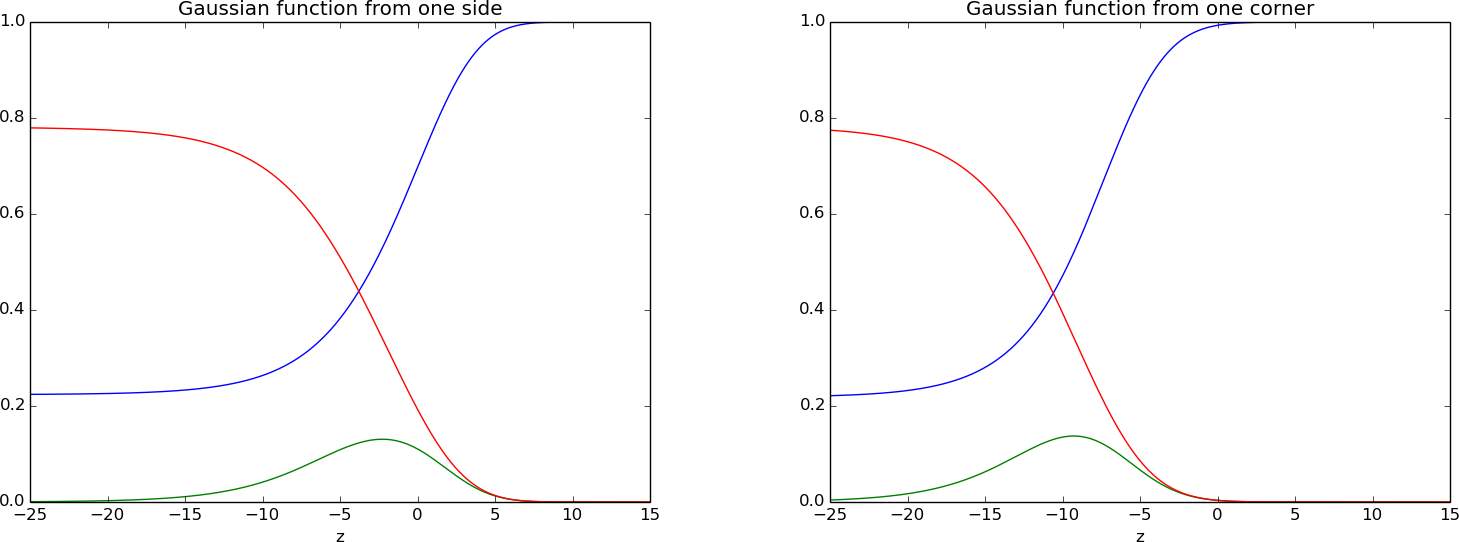
\includegraphics[width=0.8\linewidth]{plots/Trav_wave_2D.eps}}
  \caption{
  \label{fig:2D_trav_wave} Travelling wave measured at point (15,15) with two different initial values for the Infected class. The initial value is sat as a Gaussian line along (0,y) in the left plot and as a Gaussian point (0,0) in the right plot
  }
\end{figure}
%\clearpage % flush figures fig:2D_trav_wave


The shape of the two travelling waves in figure(\ref{fig:2D_trav_wave}) are similar. The only difference is the time when the wave occur. The plot for 1D wave in fig(\ref{fig:1D_tw}) has the same shape. With a closer study, the area under the function can be measured for all three cases. The result can be seen in the (\ref{table:wave_values})   

% 1D
% 1.4340793845
% 1.43143259034 dt = $1\cdot10^{-3}$, dx = 0.05
% 1.43195870243 dt = 0.0002, dx^2 = 0.000625
% 2D wave line:
% 1.43345609926 dt =0.0004, dx^2 =  0.0016
% 2D wave point:
% 1.43352971688

\label{table:wave_values}

\begin{quote}
\begin{tabular}{ccc}
\hline
\multicolumn{1}{c}{ 1D wave } & \multicolumn{1}{c}{ 2D wave line } & \multicolumn{1}{c}{ 2D wave point } \\
\hline
1.43          & 1.43          & 1.43          \\
\hline
\end{tabular}
\end{quote}

\noindent
The area in all three simulations moves towards the same area when $\Delta t$ and $\Delta x$ are reduced. The size and shape will not change by  expanding the system from 1D to 2D. But by studying the figure(\ref{fig:2D_trav_wave}), the wave occur at different times. This is caused by the distance from the start position for the Gaussian wave. The first subplot that starts with a Gaussian function along the $x=0$ axis gets a wave of infected wash along the x axis. This can be seen as a wave on the beach. Everyone that have the same distance from the ocean will be hit simultaneously. The travelling wave for the 1D simulation and the first subplot occur at the same time, because they are measured at the same distance from the starting point. The last plot is also measured at (15,15), but occur later. Since the wave starts at point (0,0), the distance to (15,15) is 21.21. This means that the wave will reach the point 6.21 time steps later. This is also reasonable by looking at the plot.    

\paragraph{Change in initial flow.}
By increasing the initial wave of \emph{Infected}, the start value of \emph{Infected} can be study. The simulation is run with the same parameters as for the three simulations above and the only difference is the initial value for the infected group. The Gaussian wave of infected are placed a point (0,0) as for right subplot in figure(\ref{fig:2D_trav_wave}).The simulation can be seen in figure(\ref{fig:initial_value}).  
% Volume ordinary = 0.3141592653589793
% Volume extreme = 157.07963267948966
% Volume under graph 1.43345609926


\begin{figure}[ht]
  \centerline{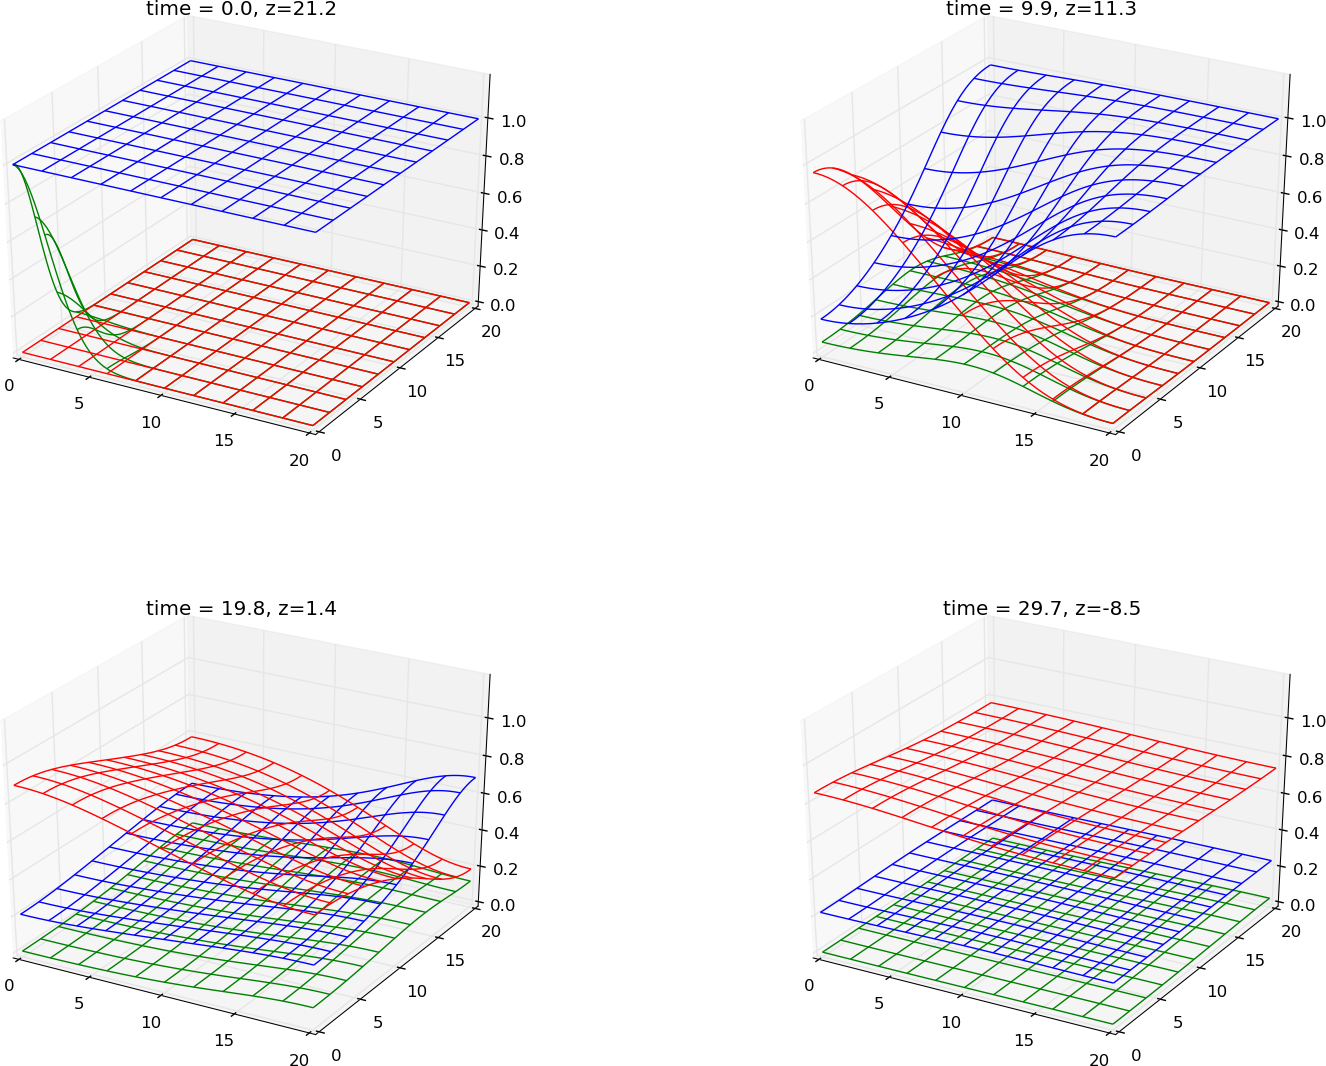
\includegraphics[width=0.8\linewidth]{plots/2D_initial_variable_sub.eps}}
  \caption{
  \label{fig:initial_value} A major flow of infected spread outwards the field. After a certain time, the wave has past the area and the number in each class stabilize.
  }
\end{figure}
%\clearpage % flush figures fig:initial_value


By measuring the travelling wave at point(15,15), the size and shape can be compared with the second subplot in figure(\ref{fig:2D_trav_wave}). The travelling wave for this simulation can be seen in figure(\ref{fig:initial_trav_wave}) and the area for the travelling wave is measured to 1.43, which is similar with the three other simulations.


\begin{figure}[ht]
  \centerline{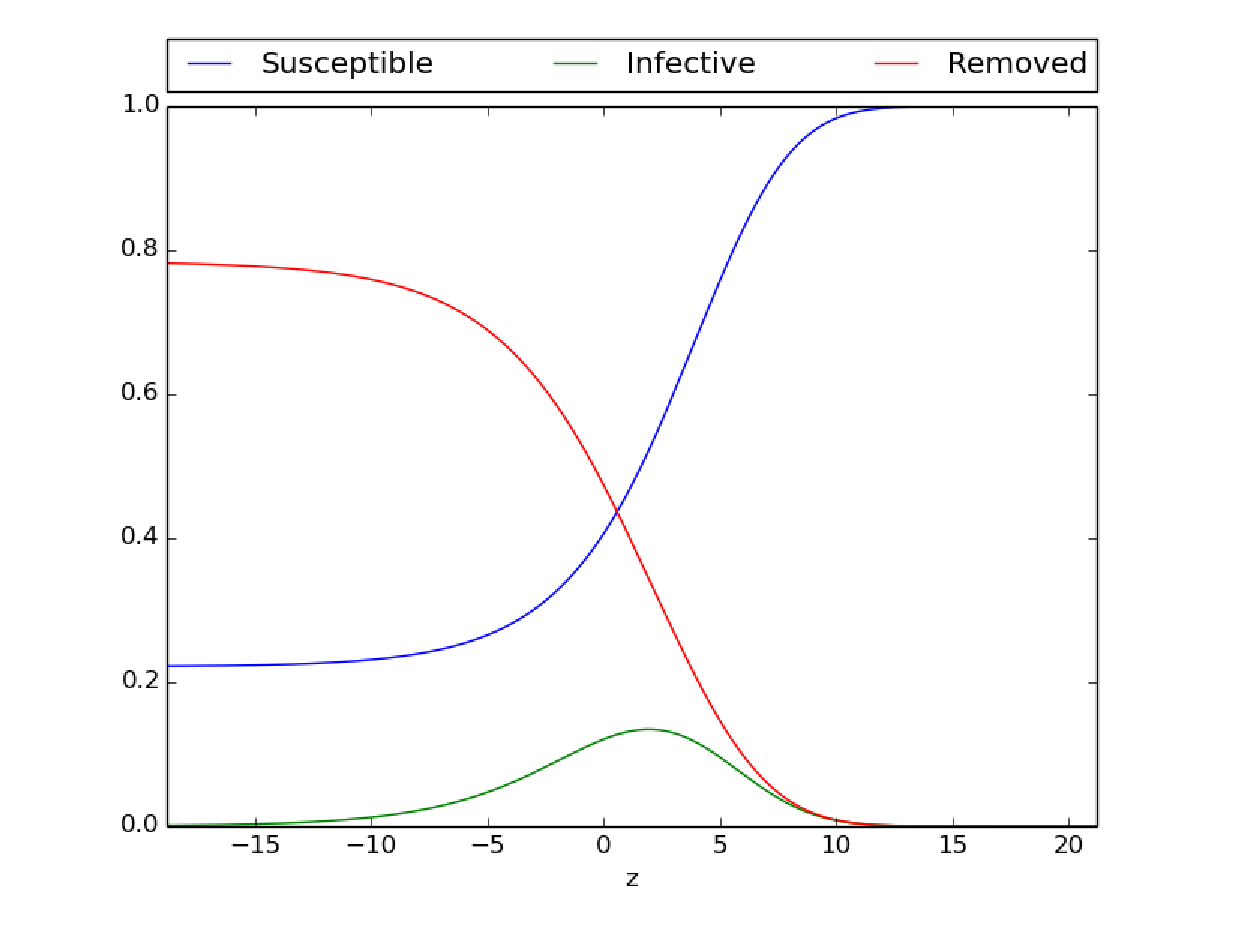
\includegraphics[width=0.8\linewidth]{plots/TW_2D_initial_z_lambda_0_5.eps}}
  \caption{
  \label{fig:initial_trav_wave} The travelling wave with a major increase of infected at the initial time.
  }
\end{figure}
%\clearpage % flush figures fig:initial_trav_wave


By increasing the initial value for the \emph{Infected} group, the size of the travelling will not be affected. But there is a difference in the time when the wave occur. In the simulation where the initial value is higher, the travelling wave reaches the measuring point (15,15) earlier. This can be explained by the idea of a ball dropped from a large height. If the ball is released or thrown to the ground, will only affect the acceleration of the ball, not the terminal velocity. After a certain time the released ball and the thrown ball will reach the same maximum speed. This is also the case for the speed of the travelling wave. 
\paragraph{Change in lambda.}
The one thing that affects the speed and size, is the $\lambda$ variable in the PDE system(\ref{eq:simple_non_PDE}). This $\lambda$ is a combination of $a$, which controls deaths among infected, $r$, which control the number of infected in a meeting between an infected and a susceptible. The last parameter in $\lambda$ is the concentration of Susceptible. By changing this parameter, the travelling wave will change in both size and shape. In figure(\ref{fig:change_lambda}), the simulation is run with four different values of $\lambda$.


\begin{figure}[ht]
  \centerline{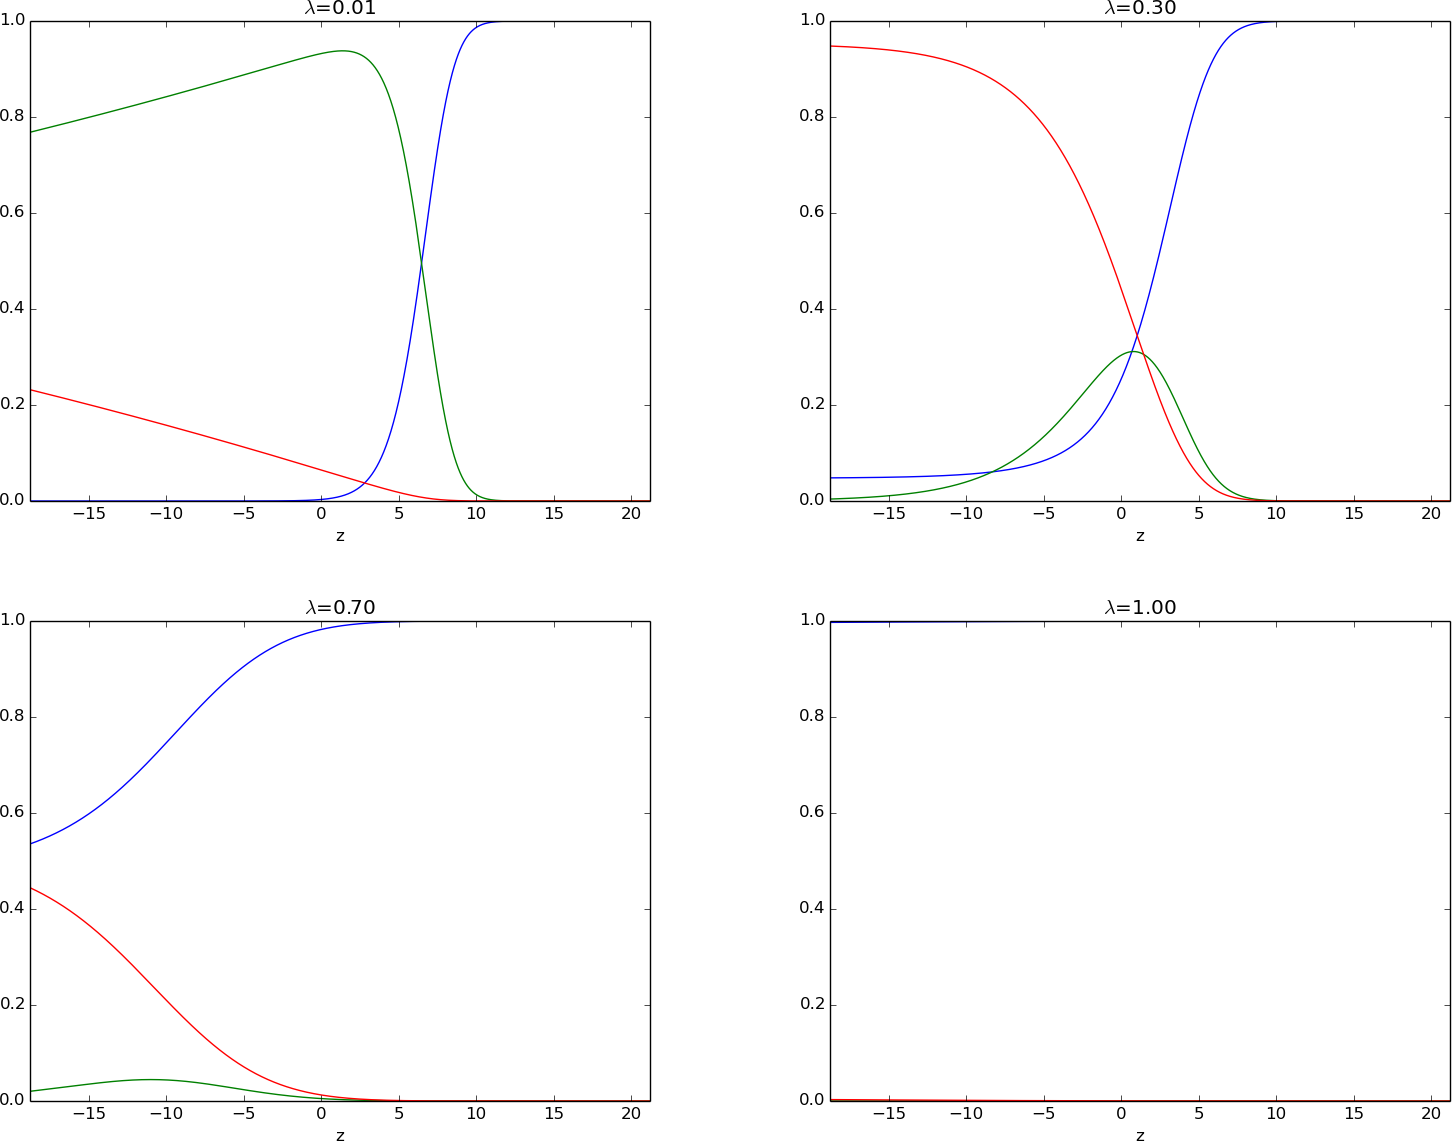
\includegraphics[width=0.9\linewidth]{plots/2D_lambda_variable.eps}}
  \caption{
  \label{fig:change_lambda} The travelling wave simulated with $\lambda$ values in the range of 0.01 to 1.
  }
\end{figure}
%\clearpage % flush figures fig:change_lambda


To understand the result in figure(\ref{fig:change_lambda}), the $\lambda $ function can be study,
\begin{equation} \label{eq:lambda}
 \lambda =\frac{a}{rS_0},
\end{equation}
A major and aggressive travelling wave is caused by $\lambda \rightarrow 0$. In figure(\ref{fig:change_lambda}), $\lambda$ is run with the value 0.01 in the first subplot. This results in a travelling wave of infected that eradicates the \emph{Susceptible} group in a short time. The wave starts to decreasing when all \emph{Susceptible} are infected. By looking at the equation(\ref{eq:lambda}), a small value is caused by a small $a$ compared to $r$ and $S_0$. If $a$ is low, this result in few deaths/immune in the infected class. This means that this class will grow and be able to infect even more from the \emph{Susceptible} class. The same thing will happen if $r$ is large. A result of this will cause an aggressive disease that infects  a major part of the population. The same result will happen if $S_0$ is large. Then there are several possible humans to infect. Therefore a outburst of a disease is more critically in a city than in the wilderness, far from other humans.
\\
\\
If $\lambda$ increases above 1, the disease will not be able to spread. The number of infected will decrease, since the number of dead/immune caused by the \emph{Infected} group is higher than the amount of \emph{Infected} humans from the \emph{Susceptible} group. After a certain time, the number of infected will die out. If $\lambda$ stays at 1, the number of infected will be equal the whole time. 

\section{Epidemic in an English Boarding School 1978}
An example from an English boarding school was presented in the previous chapter . This example was based on the book from J.D Murray \cite{murray2002mathematical}, and was modeled for a ODE system. A similar result should appear for the PDE system with same parameter values and a uniform distribution of the groups. The school had 763 students where one of the students brought a disease back to the school. The following number was used for the ODE system in chapter one. $N=763, S_0=762,I_0=1,R_0=0,\rho=202$ and $r = 2.18\cdot 10^{-3}$. 
\\
\\
The first simulation is produced with uniform distributed concentration, this is done to verify the implementation. A person is defined as one cubic. The total volume of the whole group is spread over the area. The area is sat to be 100 m x 100 m, which result in an average height of $1/10000$ m per person. This is to get an uniformed distribution. This would of course be more difficult in the real life, particular if the person should be alive. Since the \emph{Infected} group only consist of one person, the total height will be 0.0001 for the whole area. The \emph{Susceptible} group consist of 762 students and the total height in each point will be 0.0762 The simulation can be seen in the Appendix. 
\\
\\
The results from the first subplot in figure(\ref{fig:british_number}) are equal with the result from the ODE system modeled in the previous chapter.This can be seen in (\ref{table:british_number_table}). This is as expected since the diffusion term is negligible in this system and simulation is a group of separate ODE systems modeled at each point over an area.


\begin{figure}[ht]
  \centerline{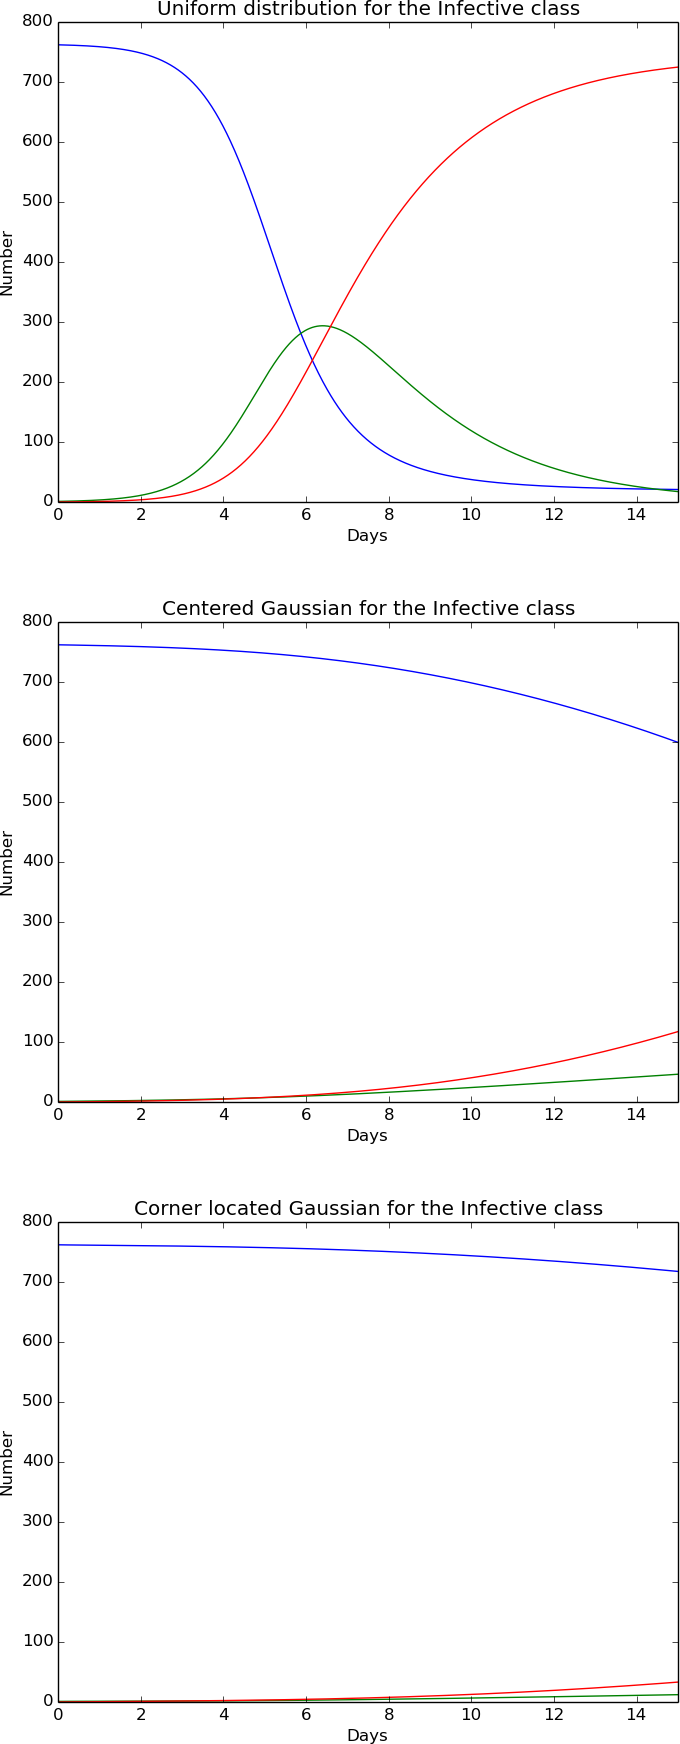
\includegraphics[width=0.8\linewidth]{plots/british_number.eps}}
  \caption{
  \label{fig:british_number} English Boarding School modeled with three different initial values for the infected student. The amount of students in each group modeled over 15 days. Subplot 1: uniform distribution. Subplot 2: The student is placed as a Gaussian function in center. Subplot 3: The student is placed as a Gaussian function in the corner (0,0).
  }
\end{figure}
%\clearpage % flush figures fig:british_number


\label{table:british_number_table}

\begin{quote}
\begin{tabular}{ccccc}
\hline
\multicolumn{1}{c}{  } & \multicolumn{1}{c}{ ODE system } & \multicolumn{1}{c}{ PDE uniform dist } & \multicolumn{1}{c}{ PDE center } & \multicolumn{1}{c}{ PDE corner } \\
\hline
5 Days              & -----------         & ------------------- & -----------         & -----------         \\
\hline
Susceptible         & 444.62              & 444.62              & 748.03              & 757.33              \\
Infective           & 209.56              & 209.56              & 7.36                & 2.35                \\
Removed             & 108.82              & 108.82              & 7.60                & 3.32                \\
\hline
10 Days             & -----------         & ------------------- & -----------         & -----------         \\
\hline
Susceptible         & 37.59               & 37.59               & 697.71              & 743.58              \\
Infective           & 117.59              & 117.59              & 24.43               & 6.66                \\
Removed             & 607.82              & 607.82              & 40.86               & 12.76               \\
\hline
15 Days             & -----------         & ------------------- & -----------         & -----------         \\
\hline
Susceptible         & 21.09               & 21.09               & 597.01              & 717.02              \\
Infective           & 17.30               & 17.30               & 46.96               & 12.37               \\
Removed             & 724.62              & 724.62              & 119.03              & 33.61               \\
\hline
\end{tabular}
\end{quote}

\noindent
% dx = 0.04
% dx^2 = 1.6E-3
% ODE = 1.5E-4

\paragraph{Introducing a Gaussian distribution of infective.}
An assumption to make is that a person is not able to be evenly distributed over an area. In this example with only one infected student at initial time, the chance of being infected increase as closer you get to the infected student. The student in placed as a Gaussian function in the middle of the school yard, to see if this affect the result. The height is sat to 1 and the volume of the Gauss function is sat to 1 cubic. The simulation can be seen in figure(\ref{fig:gauss_sub}) and the total total amount of students can be be seen in figure(\ref{fig:british_number}).


\begin{figure}[ht]
  \centerline{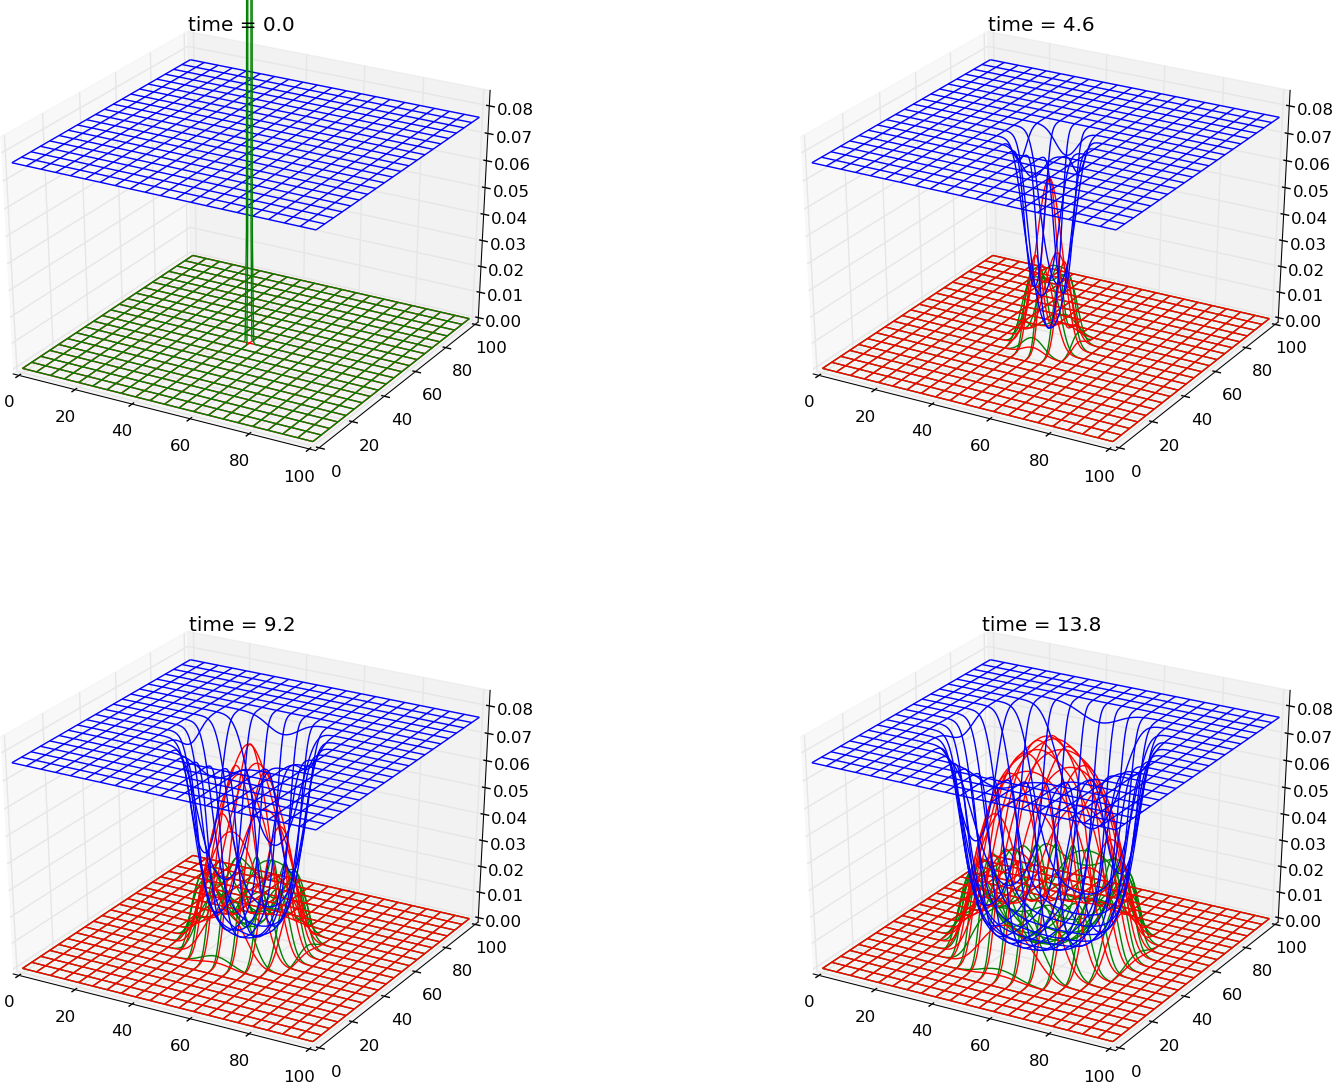
\includegraphics[width=0.8\linewidth]{plots/2D_british_school_gauss_sub.eps}}
  \caption{
  \label{fig:gauss_sub} The student is placed in the center of the school yard as a Gaussian finction with height= 1 m and volume = 1 m^3.
  }
\end{figure}
%\clearpage % flush figures fig:gauss_sub


\\
\\
The results from the uniform distributed and Gaussian distributed simulations shows variously results. The difference between the simulations is the placement of the infective. This change has a major impact. Since the only one that can be infected with the Gaussian distribution are the students close to the infective, it restrict the spread of the epidemic. While the chance of getting infected in this area is higher. The figure(\ref{fig:gauss_sub}) shows that the amount of infective quickly grow in the center, where the infected was placed. The last subplot also show that the amount of removed in the center are closed to the maximum of the initial value of Susceptible. While the students along the boundary of the school yard seems to be unaffected after 15 days. This simulation shows that the placement of the infective has a major role in the simulation.
\\
\\
The placement of the infective, here as a Gaussian function, also affects the outcome. The last subplot in Fi.(\ref{fig:british_number}) describes a simulation where the Gaussian function is placed in the corner(0,0). The total volume of the function is increased to 4 since only a quarter of the function is placed in the area. The table (\ref{table:british_number_table}) shows that the total number of infected is lower than for the centered placed Gaussian. The infected student is only able to spread the disease to a quarter of the population compared to the infected one in the center. The simulation can be seen in the Appendix.
\\
\\
If the simulations are run for a longer time, the difference between each class will decrease. After 100 days there will be about 18 susceptible students left in the uniform distributed group, compared to 25 students in both of the Gaussian groups. The simulations can be seen in the Appendix.

% !split
\section{Zombiefication}
The previous chapter studied a ODE system designed to calculate the number of humans,infected,zombies and dead during three phases in the TV series \emph{Walking Dead}. The model was based on the model from Langtangen, Mardal and Røtnes Ref.\cite{zombie-math}, with an extra term in the \emph{counter attack} phase. The ODE system from \emph{Epidemic models} can be expanded with a diffusion term in each class to make a PDE system. This can be seen in eq(\ref{eq:seland_model})  
\begin{equation} \label{eq:seland_model}
	\begin{aligned} 
	\frac{\partial S}{\partial t} =& \Sigma -(\beta+\mu \omega(t))SZ - \delta_SS +D_s\nabla^2 S \\
	\frac{\partial I}{\partial t} =& (\beta+\mu \omega(t))SZ - \varrho I - D_i\delta_II+\nabla^2 I\\
	\frac{\partial Z}{\partial t} =& \varrho I- (\alpha+\omega(t))SZ + \zeta R+D_z\nabla^2 Z\\
	\frac{\partial R}{\partial t} =& \delta_SS +\delta_II -\zeta R + (\alpha+\omega(t))SZ+D_r\nabla^2 R 
	\end{aligned}
\end{equation}
The system (\ref{eq:seland_model}) can be solved numerically by discretization. Forward Euler is used for the time derivative and Crank Nicolson for the space derivative. This is solved with the same technique as the SIR model(\ref{eq:SIR_disc}). The system can be seen in Eq. (\ref{eq:SIZR_disc})
\begin{equation} \label{eq:SIZR_disc}
	\begin{aligned}
    \frac{S^{n+1}_{i,j}-S^n_{i,j}}{\Delta t} &= \Sigma - (\beta+\mu \omega(t))S^{n}_{i,j}Z^{n}_{i,j}- \delta_S S^{n}_{i,j}+\
        D_s\left(\frac{S^{n}_{i-1,j}-2S^{n}_{i,j}+S^{n}_{i+1,j}}{\Delta x^2}+\frac{S^{n}_{i,j-1}-2S^{n}_{i,j}+S^{n}_{i,j+1}}{\Delta y^2}\right) \\
    \frac{I^{n+1}_{i,j}-I^n_{i,j}}{\Delta t} &= (\beta+\mu \omega(t))S^{n}_{i,j}Z^{n}_{i,j}-\varrho I^{n}_{i,j}- \delta_I I^{n}_{i,j}+\
        D_i\left(\frac{I^{n}_{i-1,j}-2I^{n}_{i,j}+I^{n}_{i+1,j}}{\Delta x^2}+\frac{I^{n}_{i,j-1}-2I^{n}_{i,j}+I^{n}_{i,j+1}}{\Delta y^2}\right) \\
    \frac{Z^{n+1}_{i,j}-Z^n_{i,j}}{\Delta t} &= \varrho I^{n}_{i,j}-(\alpha+\omega(t))S^{n}_{i,j}Z^{n}_{i,j}+ \zeta R^{n}_{i,j}+\
        D_z\left(\frac{Z^{n}_{i-1,j}-2Z^{n}_{i,j}+Z^{n}_{i+1,j}}{\Delta x^2}+\frac{Z^{n}_{i,j-1}-2Z^{n}_{i,j}+Z^{n}_{i,j+1}}{\Delta y^2}\right) \\
    \frac{R^{n+1}_{i,j}-R^n_{i,j}}{\Delta t} &= \delta_S S^{n}_{i,j}+\delta_I I^{n}_{i,j}-\zeta R^{n}_{i,j}+(\alpha+\omega(t))S^{n}_{i,j}Z^{n}_{i,j}
        D_r\left(\frac{R^{n}_{i-1,j}-2R^{n}_{i,j}+R^{n}_{i+1,j}}{\Delta x^2}+\frac{R^{n}_{i,j-1}-2R^{n}_{i,j}+R^{n}_{i,j+1}}{\Delta y^2}\right) 
	\end{aligned}
\end{equation}
By setting the unknown on the left, the following system (\ref{eq:SIZR_disc2}) can be solved. 
\begin{equation} \label{eq:SIZR_disc2}
	\begin{aligned}
    S^{n+1}_{i,j} &= S^n_{i,j} + \Delta t \left( \Sigma - (\beta+\mu \omega(t))S^{n}_{i,j}Z^{n}_{i,j}- \delta_S S^{n}_{i,j}+\
        D_s\left(\frac{S^{n}_{i-1,j}-2S^{n}_{i,j}+S^{n}_{i+1,j}}{\Delta x^2}+\frac{S^{n}_{i,j-1}-2S^{n}_{i,j}+S^{n}_{i,j+1}}{\Delta y^2}\right)\right) \\
    I^{n+1}_{i,j} &= I^n_{i,j} + \Delta t \left((\beta+\mu \omega(t))S^{n}_{i,j}Z^{n}_{i,j}-\varrho I^{n}_{i,j}- \delta_I I^{n}_{i,j}+\
        D_i\left(\frac{I^{n}_{i-1,j}-2I^{n}_{i,j}+I^{n}_{i+1,j}}{\Delta x^2}+\frac{I^{n}_{i,j-1}-2I^{n}_{i,j}+I^{n}_{i,j+1}}{\Delta y^2}\right)\right) \\
    Z^{n+1}_{i,j} &= Z^n_{i,j} +\Delta t \left( \varrho I^{n}_{i,j}-(\alpha+\omega(t))S^{n}_{i,j}Z^{n}_{i,j}+ \zeta R^{n}_{i,j}+\
        D_z\left(\frac{Z^{n}_{i-1,j}-2Z^{n}_{i,j}+Z^{n}_{i+1,j}}{\Delta x^2}+\frac{Z^{n}_{i,j-1}-2Z^{n}_{i,j}+Z^{n}_{i,j+1}}{\Delta y^2}\right)\right) \\
    R^{n+1}_{i,j} &= R^n_{i,j} +\Delta t \left(\delta_S S^{n}_{i,j}+\delta_I I^{n}_{i,j}-\zeta R^{n}_{i,j}+(\alpha+\omega(t))S^{n}_{i,j}Z^{n}_{i,j}
        D_r\left(\frac{R^{n}_{i-1,j}-2R^{n}_{i,j}+R^{n}_{i+1,j}}{\Delta x^2}+\frac{R^{n}_{i,j-1}-2R^{n}_{i,j}+R^{n}_{i,j+1}}{\Delta y^2}\right)\right) 
	\end{aligned}
\end{equation}
A simulation with uniform distributed classes can be done to verify the implementation of the system. The result is expected to be similar to the ODE system in the previous chapter. A zombie attack can be separated into three different phases. The first phase is short and is called the \emph{initial phase}. The humans are unfamiliar with the disease in this phase and acts quite naive to the disease. This result in a high chance of getting infected. The next phase is called \emph{Hysterical phase}. The humans are now more familiar with the situation and tries to avoid the infected ones. This result in a lower chance of getting infected. The last phase, which happens at the same time as the hysterical phase, is the counter attack. This phase is often started when humans are attacked by zombies. The following parameter that was used for simulating the first episodes in \emph{Walking Dead} will also be used here. These can be seen in (\ref{table:param_val}). By compute the system for all three phases, the value in each phase can be compared with the ones from the ODE system in the previous chapter. This will give an indication if the discretization is done correct. 

\label{table:param_val}

\begin{quote}
\begin{tabular}{cccc}
\hline
\multicolumn{1}{c}{ parameter } & \multicolumn{1}{c}{ Initial phase } & \multicolumn{1}{c}{ hysterical phase } & \multicolumn{1}{c}{ counter attack } \\
\hline
$\beta$          & 0.01155          & 0.000011         & 0.00011          \\
$\varrho$        & 1.37             & 1.5              & 1.5              \\
$\alpha$         & 0.00044          & 0.000208         & 0.000208         \\
a                & 0                & 0                & 0.0073           \\
$\sigma$         & 0                & 0                & 0.005            \\
$\mu$            & 0                & 0                & 0.14             \\
\hline
\end{tabular}
\end{quote}

\noindent
The simulation in figure(\ref{fig:zombie_three_number}) seems to match the result from the ODE system. A closer check can be done by comparing the groups in each phase. This result can be seen in (\ref{table:compare_phases_zombie}) 


\begin{figure}[ht]
  \centerline{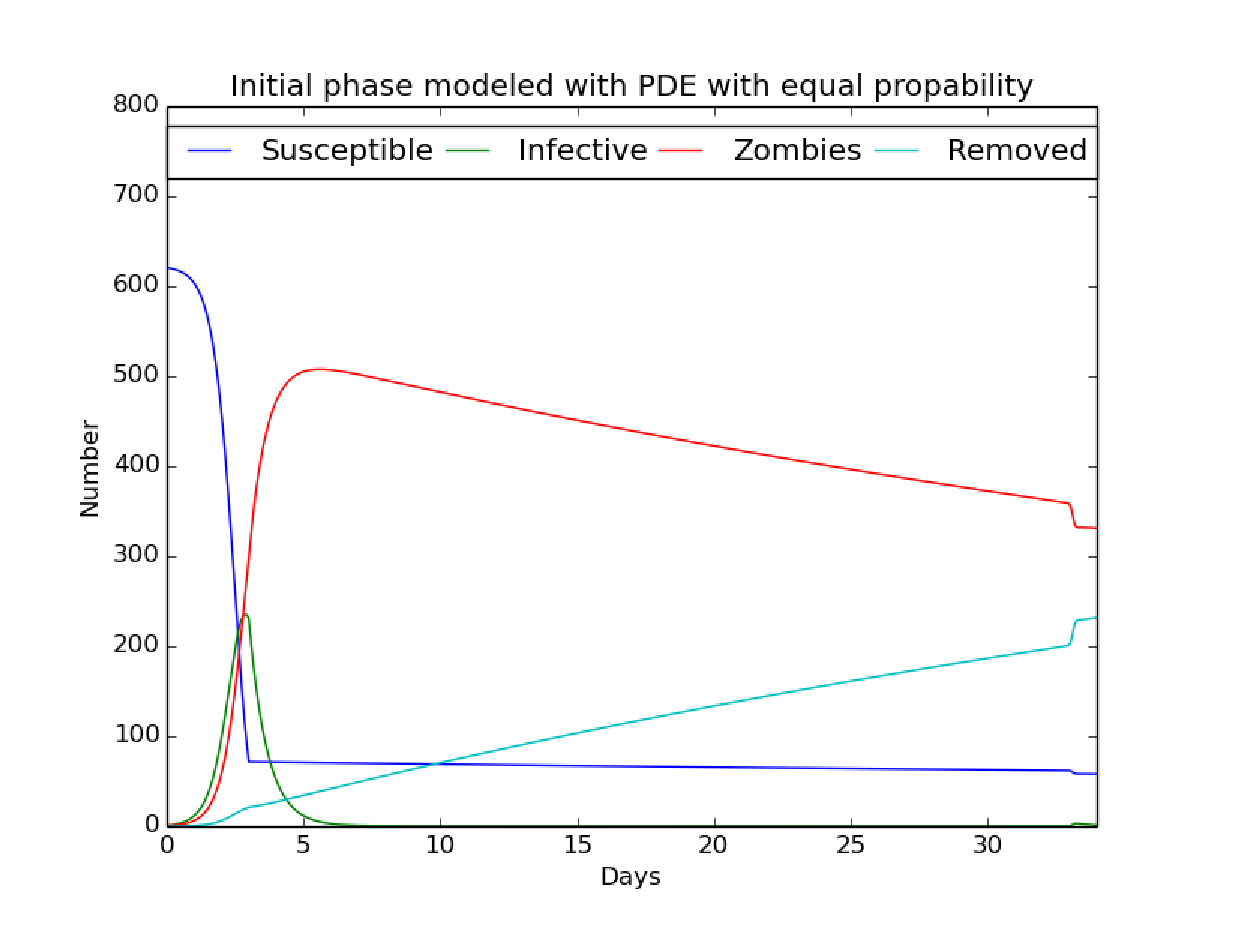
\includegraphics[width=0.8\linewidth]{plots/2D_zombie_three_phases_number.eps}}
  \caption{
  \label{fig:zombie_three_number} The system (\ref{eq:SIZR_disc2}) modeled with uniformed distributed classes. Initial values S_0 = 621,I_0 = 0, Z_0 = 0 R_0 = 0 with parameters from (\ref{table:param_val}).
  }
\end{figure}
%\clearpage % flush figures fig:zombie_three_number


The table is measured at the final time for each phase. The \emph{Initial phase} lasts for three days and the values are measured at $time=3$. The \emph{Hysterical phase} is a lasting phase, and will not stop until an eventual eradication. This is in this case measured at $time=33$, before the \emph{Counter attack}. This phase last for some hours, and is measured at $time=34$, which is a day after the attack. 

\label{table:compare_phases_zombie}

\begin{quote}
\begin{tabular}{cccc}
\hline
\multicolumn{1}{c}{  } & \multicolumn{1}{c}{ ODE system } & \multicolumn{1}{c}{ PDE uniform dist } & \multicolumn{1}{c}{ PDE gauss center } \\
\hline
Initial phase       & -----------         & ------------------- & ------------------- \\
\hline
Susceptible         & 71.3                & 71.5                & 81.12               \\
Infected            & 230.8               & 230.6               & 210.94              \\
Zombie              & 298.9               & 298.9               & 310.11              \\
Removed             & 21.0                & 21.0                & 20.60               \\
\hline
Hysterical phase    & -----------         & ------------------- & ------------------- \\
\hline
Susceptible         & 61.6                & 61.8                & 70.55               \\
Infected            & 0.3                 & 0.3                 & 0.34                \\
Zombie              & 358.6               & 357.9               & 334.33              \\
Removed             & 201.5               & 202.0               & 217.56              \\
\hline
Counter attack      & -----------         & ------------------- & ------------------- \\
\hline
Susceptible         & 57.8                & 58.2                & 66.50               \\
Infected            & 1.2                 & 1.2                 & 1.23                \\
Zombie              & 331.8               & 331.1               & 305.86              \\
Removed             & 231.3               & 231.7               & 249.19              \\
\hline
\end{tabular}
\end{quote}

\noindent
These results shows that the PDE system gives the same result as for the ODE. The small error can be explained by $\Delta t$ and $\Delta x$, and can be reduced to the expected error by decreasing these values.

% #
% #
% #
% #


\paragraph{Where does the infected one arises.}
In the previous section \emph{English boarding school}, the placement of the infected was proven to have a major influence on the result. But here the \emph{Susceptible} was uniformed distributed over the schoolyard. Based on the study of \emph{Walking Dead}, the amount in each class was seen in three different areas where Rick went by. Only by studying the TV series, it is hard to decide the geograpic distance between these three places. Therefore they have been placed with a certain distance from each other. The following simulation is done on a grid with size(40 x 40) with the following placement on the towns. Small town(6,6) with size 21, middle town(12,25) with size 200 and large town(25,12) with size 400. Since these values was based on the humans and zombies seen in the series, these can be scaled up. The total population can be scaled up by 1000, so the large town can be seen as an area with a population of 400 000. The length can be measured in kilometre. Then the distance between the middle and large town will be 18.38 km. Compared to the distance between Oslo and Bærum(Sandvika) which is 15 km, the simulation can be seen as rough estimate of the area around Oslo. Of course with a frozen fjord and similar mobility for the whole area.  
\\
\\
The diffusion term describe the diffusion for each class. This can be seen as the speed for each group. If the diffusion constant is large, the flow towards equilibrium will go faster. The values have been sat as follows. 
\begin{itemize}
\item $D_s=1$, The \emph{Susceptible} has a basic moving speed. The other classes are based on the speed of a healthy human.

\item $D_i=0.5$, The \emph{Infected} are often injured caused by recently fights. This affects their mobility

\item $D_z=0.9$, The average moving speed for a zombie. There are zombies with the mobility of a human, but there are also cases where zombies drag them self forward with only one arm. This result in a major difference in speed and therefore a lower average speed for the zombies.

\item $D_r=0$, The removed are here seen as dead, therefore there are no mobility.
\end{itemize}

\noindent
\\
\\
The parameters from (\ref{table:param_val}) will be used here, and the three phases will be modeled as shown for the uniformed distributed PDE system. The values will be used for three different simulations with similar initial value for the different classes. The initial values can be seen in figure(\ref{fig:initial_value_susceptible}) and are based on the data given above. The difference in the three different simulations will be the placement of the zombie at initial time. The zombie will be placed in center of the small, middle and large town.


\begin{figure}[ht]
  \centerline{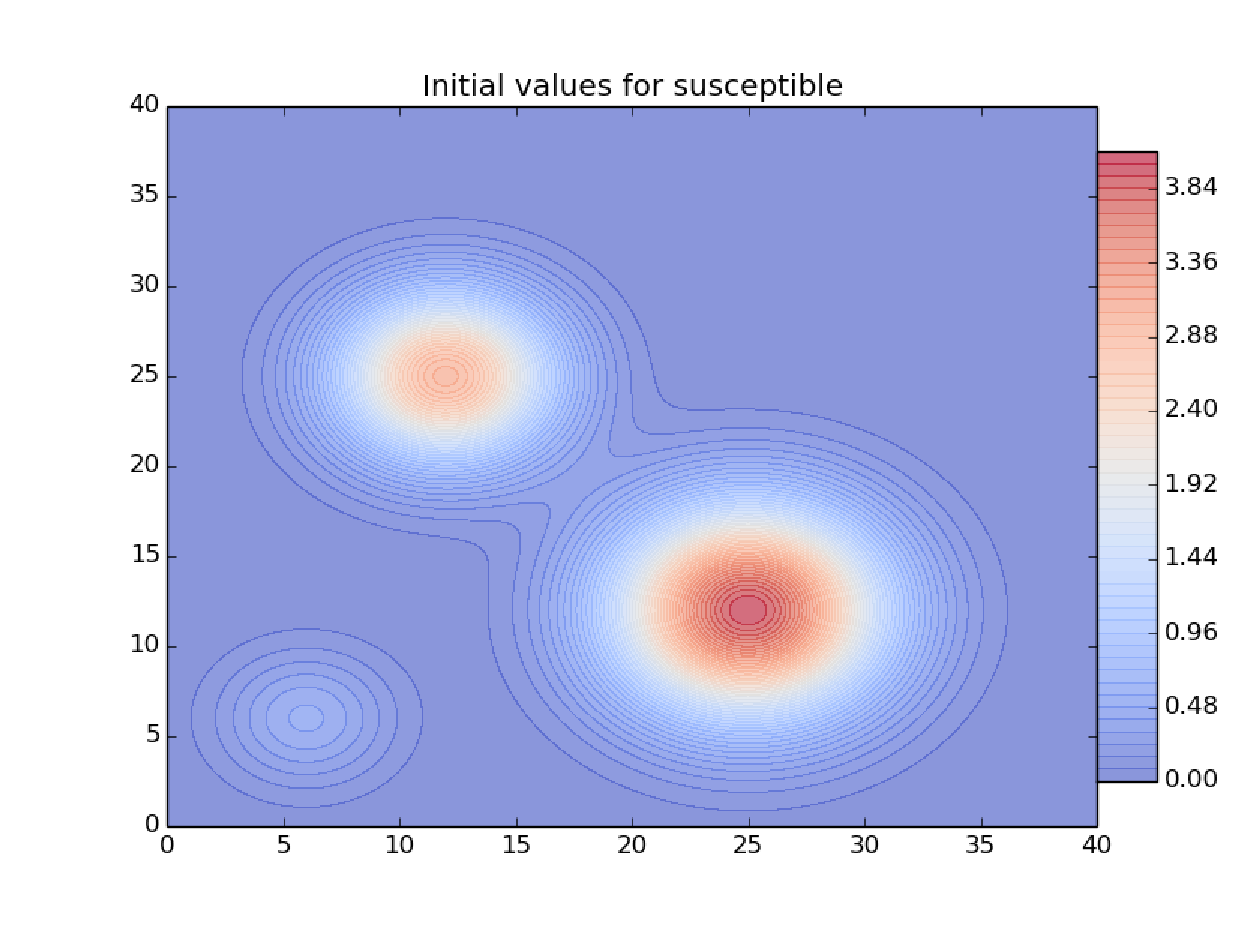
\includegraphics[width=0.8\linewidth]{plots/initial_value_susceptible.eps}}
  \caption{
  \label{fig:initial_value_susceptible} The initial value for the \emph{Susceptible} group for three simulations. Small group(6,6) with volume 21, middle group(12,25) with volume 200 and large group(25,12) with volume 400. All three groups are build up with a Gaussian function
  }
\end{figure}
%\clearpage % flush figures fig:initial_value_susceptible


The figure(\ref{fig:large_town}) shows the simulation where the zombie is placed in the large town. The simulations of the small and middle town can be seen in the Appendix. The four subplots are from the different phases that arise under a zombie attack. The different classes have the same color as introduced in figure(\ref{fig:zombie_three_number}). It is a challenge to separate the three groups \emph{Infected},*Zombie* and \emph{Removed}, since they all have a low value at initial time. The development of the amount can easier be seen in the figure(\ref{fig:compare_towns}), which also shows the result from the small and middle group. Since the amount of \emph{Susceptible} is quite low in the small town where the Zombie arise, the disease is not able to infect to many before the society has moved to the next phase. Assuming that the broadcasting about the disease works okay for the first days. This result in a eradication of the disease in about a month. The table(\ref{table:compare_phases_zombie}) shows that the number of zombies decrease towards zero after a month. 


\begin{figure}[ht]
  \centerline{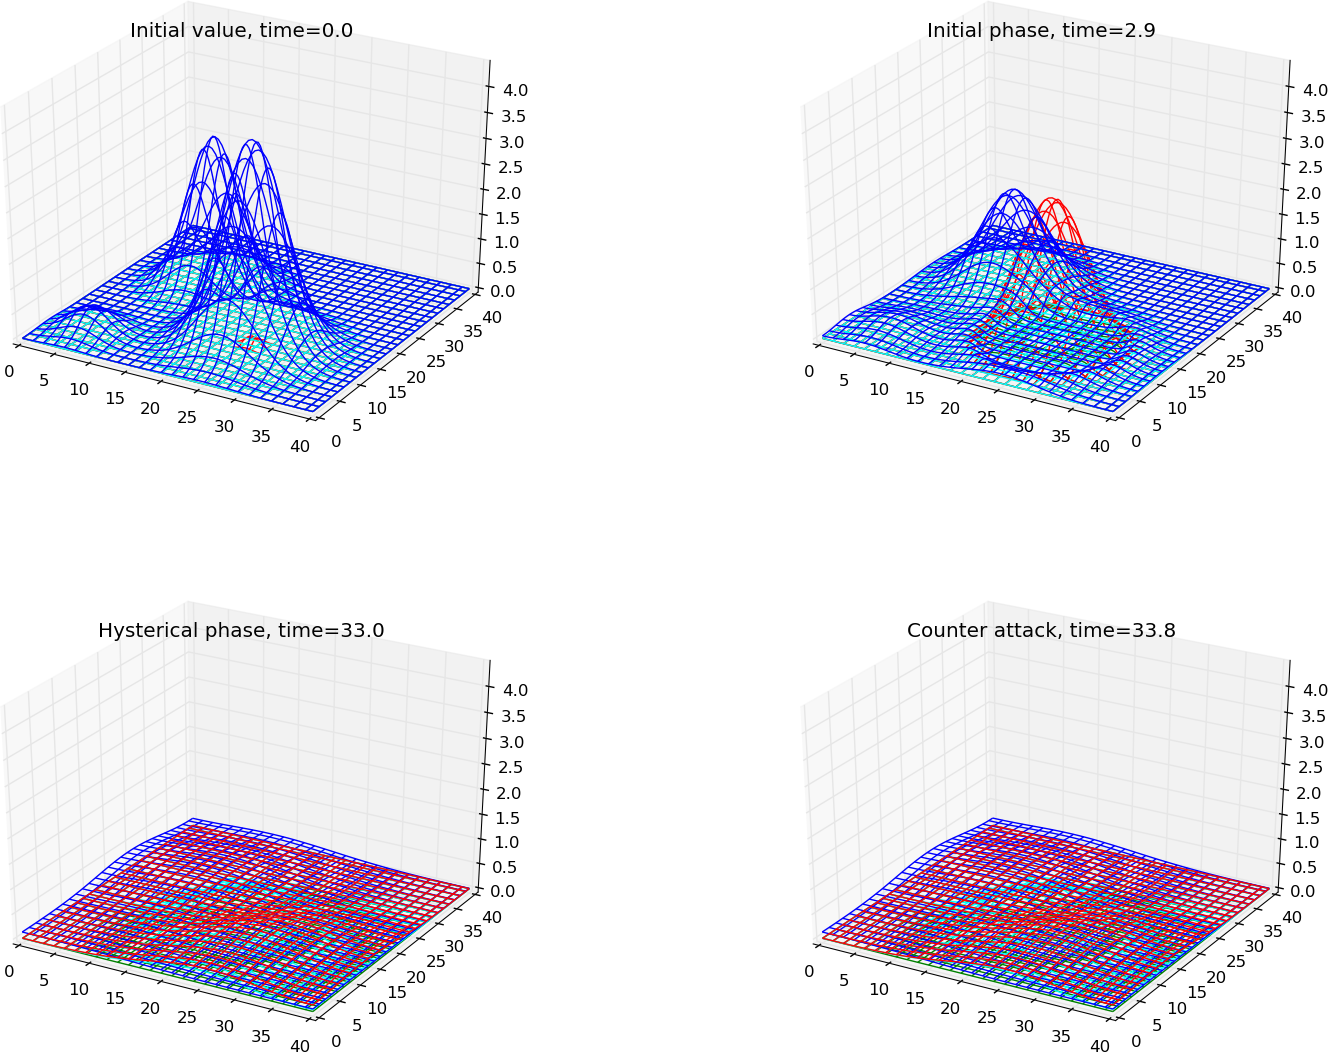
\includegraphics[width=0.8\linewidth]{plots/2D_zombie_three_phases_zombie_large_town_2_sub.eps}}
  \caption{
  \label{fig:large_town} \emph{Walking Dead} simulated with the infected at initial time in the large town. Subplots shown at each phase.
  }
\end{figure}
%\clearpage % flush figures fig:large_town


By placing the Zombie in the middle town, the amount of zombies increase to a much higher level. The amount can be seen as the second sub figure in figure(\ref{fig:compare_towns}). The damages are higher and after a month the total population of \emph{Susceptible} is reduced to 427. The last calculation done in the large town (\ref{fig:large_town}) shows major damages. Here the amount of \emph{Zombie} increase above the number of \emph{Susceptible}. The \emph{Infected} class also increase to above 100 after a couple of days in the infected phase. This can be explained by the high number of meetings between susceptible and zombies. By studying the second subplot in figure(\ref{fig:large_town}), the zombies are grouped in the large town, while the middle and small town mostly consist of \emph{Susceptible}. By counting the loss of \emph{Susceptible} during the first phase, the table shows that this amount correspond to the size of the towns where the zombie was placed, given by the number 17,188 and 362 with the zombie in the small,middle and large group. The percent is highest in the middle town with 94 %. The percent in the large and small group are 90 % and 81 %. The simulation in the middle town has the highest percent because the large town also gets infected. These towns are coupled together, and the zombiefication is able to spread. The small town, which can be seen as Nesodden, has the lowest percent. This is not able to spread to the other towns, and cause less damages.  


\begin{figure}[ht]
  \centerline{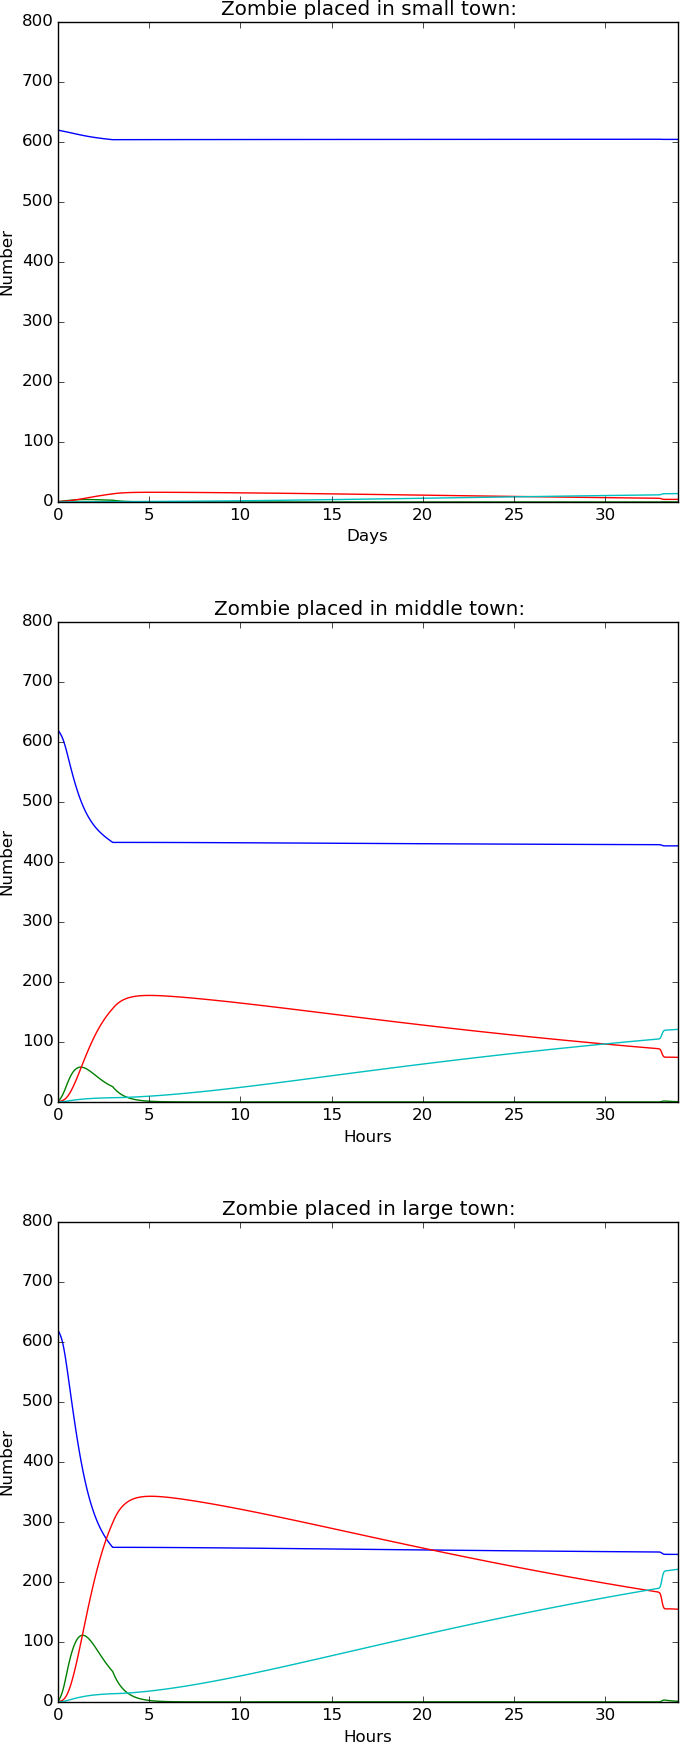
\includegraphics[width=0.8\linewidth]{plots/2D_compare_towns.eps}}
  \caption{
  \label{fig:compare_towns} The values for each group counted during 34 days in \emph{Walking Dead}. Initial phase from day 0 to day 3, Hysterical phase from day 3 to day 33 and Counter attack from day 33 to day 34.
  }
\end{figure}
%\clearpage % flush figures fig:compare_towns


The result from the uniformed distributed simulation still is much higher for the \emph{Zombie} class then for the large town. This shows that by using the parameters from the ODE system in a geographic area give no sense. A realistic assumption is that a zombie is restricted to a given area. Therefore the parameters will not be equal for all. The chance of getting infected is much higher if a susceptible is closed to an infected. There is also a greater chance of getting infected if the susceptible stay in a crowded area.

\label{table:compare_phases_zombie}

\begin{quote}
\begin{tabular}{cccc}
\hline
\multicolumn{1}{c}{  } & \multicolumn{1}{c}{ Small town } & \multicolumn{1}{c}{ Middle town } & \multicolumn{1}{c}{ Large } \\
\hline
Initial phase       & -----------         & ------------------- & ------------------- \\
\hline
Susceptible         & 603.74              & 433.22              & 259.20              \\
Infected            & 2.96                & 25.51               & 50.94               \\
Zombie              & 13.79               & 155.27              & 297.24              \\
Removed             & 0.66                & 7.16                & 13.78               \\
\hline
Hysterical phase    & -----------         & ------------------- & ------------------- \\
\hline
Susceptible         & 604.42              & 429.35              & 251.14              \\
Infected            & 0.03                & 0.18                & 0.35                \\
Zombie              & 6.25                & 87.31               & 178.45              \\
Removed             & 12.14               & 106.00              & 192.90              \\
\hline
Counter attack      & -----------         & ------------------- & ------------------- \\
\hline
Susceptible         & 604.21              & 427.45              & 247.33              \\
Infected            & 0.08                & 0.59                & 1.17                \\
Zombie              & 4.49                & 73.70               & 151.44              \\
Removed             & 14.11               & 121.16              & 222.96              \\
\hline
\end{tabular}
\end{quote}

\noindent
\subsection{Lock in different areas}
To model a realistic zombie attack, humans ability to think logic is crucial in the fight. The moving speed was presented as a factor in the previous section. Another important skill that the \emph{Susceptible} class hold, is the ability to decide the safety of an area. In the TV series \emph{Walking Dead}, the humans build barricades to keep the zombies outside. This give the \emph{Susceptible} class free areas where they can stay. This idea can be transfer to the PDE system by rewrite the system (\ref{eq:seland_model}) with spatial dependent diffusion term. The diffusion constant $D_u$ is now replaced with a diffusion function $\gamma_u(x)$ for $u= S,I,Z,R$ which is spatial discretized. Since a diffusion equation always goes towards equilibrium, this rewriting will only slow down/stop the selected class to diffuse into an area. In this case the \emph{Zombie} class to diffuse into the buildings. 

\begin{equation} \label{eq:seland_model_diff}
    \begin{aligned} 
    \frac{\partial S}{\partial t} =& \Sigma -(\beta+\mu \omega(t))SZ - \delta_SS +\nabla(\gamma_S(x) \nabla S) \\
    \frac{\partial I}{\partial t} =& (\beta+\mu \omega(t))SZ - \varrho I - D_i\delta_II+\nabla(\gamma_I(x) \nabla I)\\
    \frac{\partial Z}{\partial t} =& \varrho I- (\alpha+\omega(t))SZ + \zeta R+\nabla(\gamma_Z(x) \nabla Z)\\
    \frac{\partial R}{\partial t} =& \delta_SS +\delta_II -\zeta R + (\alpha+\omega(t))SZ+\nabla(\gamma_R(x) \nabla R) 
    \end{aligned}
\end{equation}

The diffusion term is the difference between this system and system(\ref{eq:seland_model}). The discretization can be shown for for a general $\gamma$. This will be similar for all classes. A Crank Nicolson discretization is used in space.

\begin{equation} \label{eq:gamma}
    \begin{aligned}
    &=\nabla(\gamma(x) \nabla S) \\
    &=(\gamma(x) S_x)_x+(\gamma(x) S_y)_y \\
    &= \left(\gamma(x) \frac{S^{n}_{i+1/2,j}-S^{n}_{i-1/2,j}}{\Delta x}\right)_x+\left(\gamma(x) \frac{S^{n}_{i,j+1/2}-S^{n}_{i,j-1/2}}{\Delta y}\right)_y \\
    &= \left(\frac{\gamma(x_{i+1/2,j})(S^{n}_{i+1,j}-S^{n}_{i,j})-\gamma(x_{i-1/2,j})(S^{n}_{i,j}-S^{n}_{i-1,j})}{\Delta x^2}\right)+\left(\frac{\gamma(x_{i,j+1/2})(S^{n}_{i,j+1}-S^{n}_{i,j})-\gamma(x_{i,j-1/2})(S^{n}_{i,j}-S^{n}_{i,j-})}{\Delta y^2}\right)
    \end{aligned}
\end{equation}
Since the calculation is based on spatial points, the values inside the function of $\gamma$ need to be adjusted. This can be done by an aritmetic mean. This can be seen in eq(\ref{eq:arith_mean}). The writing $q_{i+1/2}$ is used for the function $q(x_{i+1/2})$ with $x_{i+1/2} = x_i + 1/2 \Delta x$
\begin{equation} \label{eq:arith_mean}
q_{i+1/2} \approx \frac{1}{2}(q_i +q_{i+1})
\end{equation}
This arithmetic mean can be inserted for all $\gamma$'s in the system.By cleaning up, the system can be expressed.
\begin{equation} \label{eq:SIZR_disc3}
	\begin{aligned}
    S^{n+1}_{i,j} &= S^n_{i,j} + \Delta t \left( \Sigma - (\beta+\mu \omega(t))S^{n}_{i,j}Z^{n}_{i,j}- \delta_S S^{n}_{i,j}+\
        \frac{1}{2\Delta x^2}\left(\gamma_S(x_{i-1,j})(S^{n}_{i-1,j}-S^{n}_{i,j})+\gamma_S(x_{i,j})(S^{n}_{i-1,j}-2S^{n}_{i,j}+S^{n}_{i+1,j})+\gamma_S(x_{i+1,j})(-S^{n}_{i,j}+S^{n}_{i+1,j})\right)+\
        \frac{1}{2\Delta y^2}\left(\gamma_S(x_{i,j-1})(S^{n}_{i,j-1}-S^{n}_{i,j})+\gamma_S(x_{i,j})(S^{n}_{i,j-1}-2S^{n}_{i,j}+S^{n}_{i,j+1})+\gamma_S(x_{i,j+1})(-S^{n}_{i,j}+S^{n}_{i,j+1})\right)\right)\\
    I^{n+1}_{i,j} &= I^n_{i,j} + \Delta t \left((\beta+\mu \omega(t))S^{n}_{i,j}Z^{n}_{i,j}-\varrho I^{n}_{i,j}- \delta_I I^{n}_{i,j}+\
        \frac{1}{2\Delta x^2}\left(\gamma_I(x_{i-1,j})(I^{n}_{i-1,j}-I^{n}_{i,j})+\gamma_I(x_{i,j})(I^{n}_{i-1,j}-2I^{n}_{i,j}+I^{n}_{i+1,j})+\gamma_I(x_{i+1,j})(-I^{n}_{i,j}+I^{n}_{i+1,j})\right)+\
        \frac{1}{2\Delta y^2}\left(\gamma_I(x_{i,j-1})(I^{n}_{i,j-1}-I^{n}_{i,j})+\gamma_I(x_{i,j})(I^{n}_{i,j-1}-2I^{n}_{i,j}+I^{n}_{i,j+1})+\gamma_I(x_{i,j+1})(-I^{n}_{i,j}+I^{n}_{i,j+1})\right)\right)\\
    Z^{n+1}_{i,j} &= Z^n_{i,j} +\Delta t \left( \varrho I^{n}_{i,j}-(\alpha+\omega(t))S^{n}_{i,j}Z^{n}_{i,j}+ \zeta R^{n}_{i,j}+\
        \frac{1}{2\Delta x^2}\left(\gamma_Z(x_{i-1,j})(Z^{n}_{i-1,j}-Z^{n}_{i,j})+\gamma_Z(x_{i,j})(Z^{n}_{i-1,j}-2Z^{n}_{i,j}+Z^{n}_{i+1,j})+\gamma_Z(x_{i+1,j})(-Z^{n}_{i,j}+Z^{n}_{i+1,j})\right)+\
        \frac{1}{2\Delta y^2}\left(\gamma_Z(x_{i,j-1})(Z^{n}_{i,j-1}-Z^{n}_{i,j})+\gamma_Z(x_{i,j})(Z^{n}_{i,j-1}-2Z^{n}_{i,j}+Z^{n}_{i,j+1})+\gamma_Z(x_{i,j+1})(-Z^{n}_{i,j}+Z^{n}_{i,j+1})\right)\right)\\
    R^{n+1}_{i,j} &= R^n_{i,j} +\Delta t \left(\delta_S S^{n}_{i,j}+\delta_I I^{n}_{i,j}-\zeta R^{n}_{i,j}+(\alpha+\omega(t))S^{n}_{i,j}Z^{n}_{i,j}\right)
	\end{aligned}
\end{equation}
The diffusion term for the \emph{Removed} class is take away, since dead people are not able to move. This system looks quite messy, but it is straight forward to calculate. All values on the right side are known values and the system is easy to solve. Now every point will be controlled by its diffusion constant. This makes it easier to control the flow in each class. With a high diffusion constant, the diffusion will spread fast. When the diffusion constant goes towards zero, the flow will decrease towards zero flow. This will result in a set of ODE systems modeled for each point.

\paragraph{Ten minutes at Frederikkeplassen.}
Frederikkeplassen at the university is a possible area for an upcoming zombie attack. This simulation will try to model a ten minutes sequence with the diffusion parameter added in this section. Since students often learn and interact fast, they will only use three minutes before they realise the danger and goes into the \emph{Hysterical phase}. A map of Frederikkeplassen is used to define the safe and non save areas. The buildings are set as areas where only the \emph{Susceptible} are allowed to move. This is done by setting the diffusion constant to zero for the \emph{Zombie} and \emph{Infected} class. Since the buildings are safe spots for the \emph{Susceptible}, an idea would be to express this in the diffusion term by forcing the \emph{Susceptible} for other areas into the buildings. This more difficult, since the concentrations in each class wants to go towards equilibrium. A way to delay this process is by setting the diffusion constant to be low in the buildings and high outside. This will result in a fast diffusion in the open areas and a slow inside the buildings. 


\begin{figure}[ht]
  \centerline{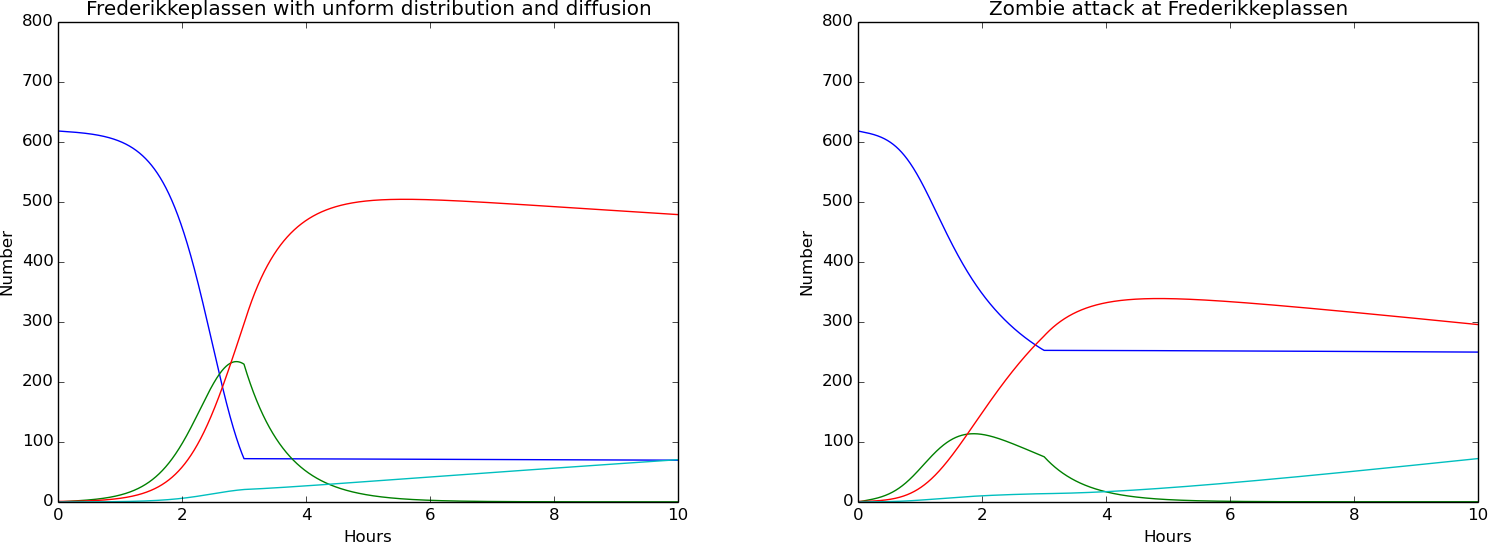
\includegraphics[width=0.8\linewidth]{plots/2D_compare_Frederikke.eps}}
  \caption{
  \label{fig:frederikke_numbers} The amount in each group for two simulations of Frederikkeplassen modeled same parameters for 10 minutes/hours. a)Plot with uniformed distributed groups and same diffusion constants for all classes. b)Plot based on figure(\ref{fig:frederikke_free_area}) with different initial values for each group.
  }
\end{figure}
%\clearpage % flush figures fig:frederikke_numbers


Two simulations have been done on Frederikkeplassen. The amount in each group can be seen in figure(\ref{fig:frederikke_numbers}). The first simulation has a solution based on the ODE system, with uniformed distributed classes, equal diffusion constants and no free areas for the \emph{Susceptible}. The second simulation is model with three groups of \emph{Susceptible}, as in the previous Section. The small group with 21 students is placed at point(4,4), the middle group with 200 students is placed at point(15,8) and the large group with 400 students is placed at point(8,13). The zombie is placed at point(8,10). The $\gamma(x)$ is sat to zero in the buildings for the \emph{Zombie} and \emph{Infected} class, and one in the rest of the area. For the \emph{Susceptible} class, $\gamma(x)$ is sat to 0.1 in the buildings, which causing slow diffusion. In the areas, the $\gamma(x)$ is sat to 5 for the \emph{Susceptible}. The desired idea is to push them into  the buildings, but this will only happen if there is a lower concentration inside the buildings. Therefore this will not reflect a realistic flow of a \emph{Susceptible} population. This simulation can be seen in figure(\ref{fig:frederikke_free_area})  


\begin{figure}[ht]
  \centerline{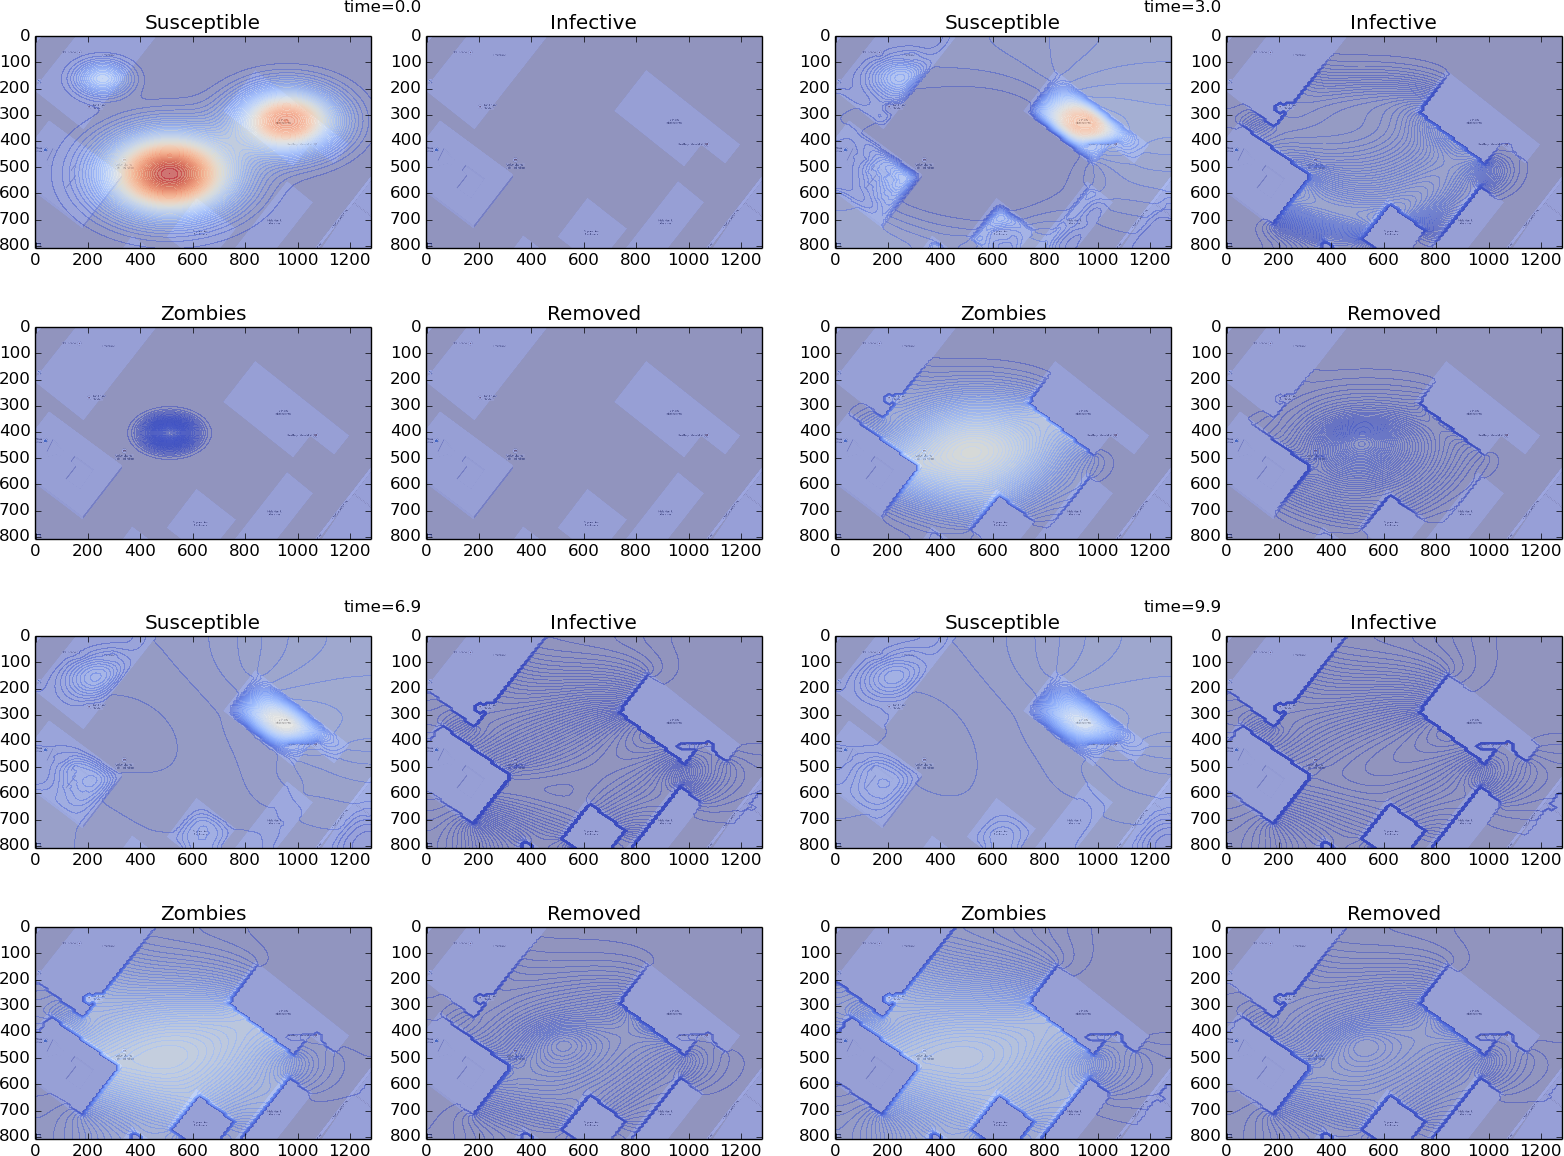
\includegraphics[width=0.8\linewidth]{plots/2D_Frederikke_contourf_sub.eps}}
  \caption{
  \label{fig:frederikke_free_area} Frederikkeplassen modeled with free areas for the \emph{Susceptible} group. The diffusion function $\gamma(x)$ is sat to zero for the \emph{Zombie} and \emph{Infected} group in the buildings. The zombie at initial time is placed in the center of Frederikkeplassen
  }
\end{figure}
%\clearpage % flush figures fig:frederikke_free_area


The numbers in table(\ref{table:frederikke_table}) shows that the three first minutes are the crucial phase. The number after three minutes shows only that only 72 humans survived the attack in the uniformed solution,compared to 252 in the free areas, even more in the simulation with the random placement. But the number of \emph{Susceptible} is quite similar measured at $t=3$. But at $t=7$, the difference is major. This can be explained by looking at figure(\ref{fig:frederikke_free_area}) and the building with the middle group placed inside. When the zombie starts attacking at $t=0$, the large group is exposed. This group is placed close to the zombie and the position is in an open area. The zombie can attack right away and the number of infected and zombies increase fast. In the two first minutes, a major part of the large group is infected and the \emph{Zombie} group starts to spread. After 2-3 minutes, the group has reaced the buildings with the middle group. But they are not able to diffuse in. Since the diffusion variable is quite low inside the building for the \emph{Susceptible}, it takes time before the group diffuses out. Maybe the right diffusion value along the buldings would be 0, to avoid any leakage. This will again cause the problem that no \emph{Susceptible} can move in. It is also reasonable to think that the \emph{Susceptible} group needs to diffuse out. The lack of suplies would force them out.



% #
% #

\label{table:frederikke_table}

\begin{quote}
\begin{tabular}{cccc}
\hline
\multicolumn{1}{c}{  } & \multicolumn{1}{c}{ Uniform distribution } & \multicolumn{1}{c}{ Free areas } & \multicolumn{1}{c}{ Random placement } \\
\hline
3 Minutes                   & --------------------------- & ---------------             & ----------------            \\
\hline
Susceptible                 & 72.23                       & 252.72                      & 524.77                      \\
Infected                    & 229.65                      & 75.69                       & 26.07                       \\
Zombie                      & 296.67                      & 276.55                      & 66.51                       \\
Removed                     & 20.84                       & 13.94                       & 3.66                        \\
\hline
7 Minutes                   & --------------------------- & ---------------             & ----------------            \\
\hline
Susceptible                 & 70.78                       & 251.35                      & 524.23                      \\
Infected                    & 0.83                        & 0.51                        & 0.20                        \\
Zombie                      & 498.72                      & 325.54                      & 81.88                       \\
Removed                     & 49.12                       & 41.26                       & 14.80                       \\
\hline
10 Minutes                  & --------------------------- & ---------------             & ----------------            \\
\hline
Susceptible                 & 69.69                       & 249.84                      & 523.61                      \\
Infected                    & 0.25                        & 0.38                        & 0.16                        \\
Zombie                      & 479.00                      & 295.71                      & 69.67                       \\
Removed                     & 70.55                       & 72.36                       & 27.77                       \\
\hline
\end{tabular}
\end{quote}

\noindent
\paragraph{random distribution.}
This random distribution of \emph{Susceptible} and \emph{Zombie} is based with the idea of the next chapter. The \emph{Susceptible} group is random placed over the area by random draw the height of each point. The volume is similar to the two other simulations in table(\ref{table:frederikke_table}) and the zombie is random placed. The simulation has the same $\gamma(x)$ as the simulation of the free areas, but the result is different. This simulation was done a couple of times, and resulted in different solutions each time. The position of the zombie had a major influece on the result. If this was placed in the center, the amount of \emph{Infeced} and \emph{Zombie} was larger than in the corner of the plot. Therefore it is difficult to compare this result with the two other simulations. But the amount of \emph{Susceptible} after 3 minues was never under the amount in for the simulation with free areas.  


\begin{figure}[ht]
  \centerline{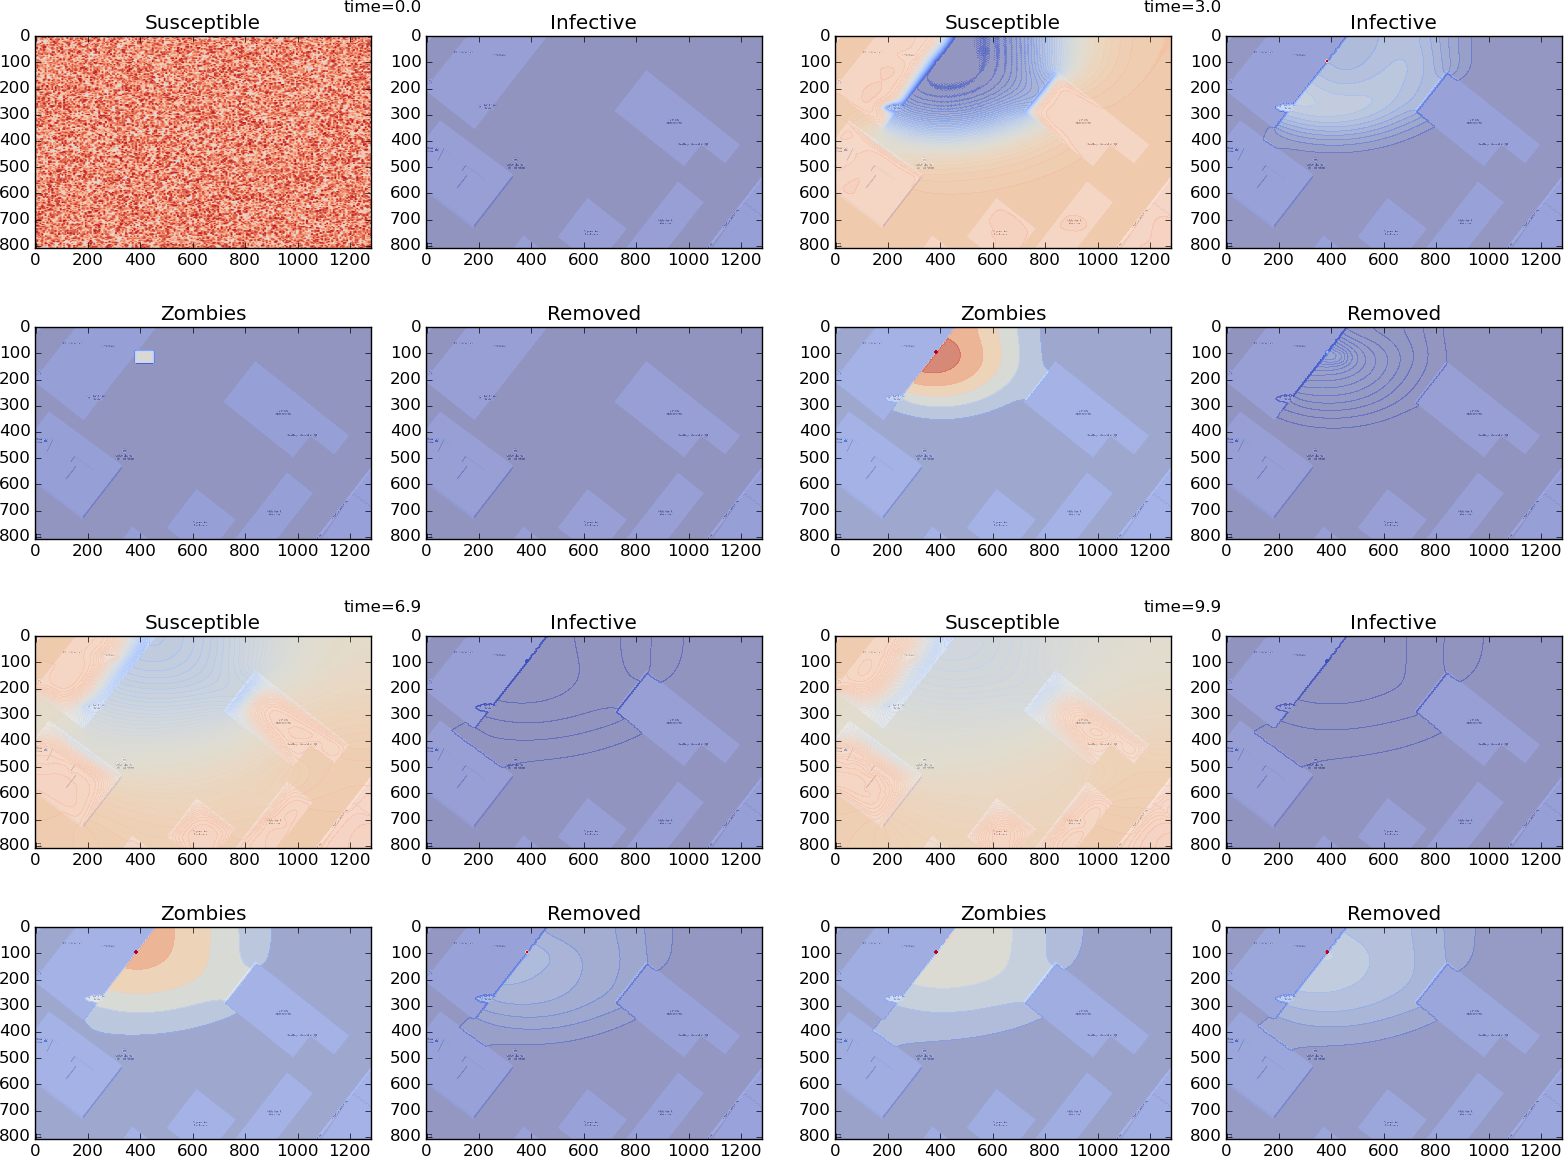
\includegraphics[width=0.8\linewidth]{plots/2D_Frederikke_random_contourf_sub.eps}}
  \caption{
  \label{fig:frederikke_random} Random position of the \emph{Susceptible} and \emph{Zombie} class. Simulated with free areas inside the buildings.
  }
\end{figure}
%\clearpage % flush figures fig:frederikke_random




% !split
\section{Appendix}
\paragraph{Sympy to find manufactured solution.}
\bpycod
>>> from sympy import *
>>> x,t,lam = symbols('x t lam')
>>> def s_simple(x,t):
...     return cos(pi*x)*t
... 
>>> def i_simple(x,t):
...     return cos(pi*x)*t
... 
>>> def r_simple(x,t):
...     return cos(pi*x)*t
... 
>>> for x_point in 0,1:
...     print "s_x(%s,t): ", % x_point,
>>> for x_point in 0,1:
...     print "s_x(%s,t): " % x_point,
...     print diff(s_simple(x,t),x).subs(x,x_point).simplify()
...     print "i_x(%s,t): " % x_point,
...     print diff(i_simple(x,t),x).subs(x,x_point).simplify()
...     print "r_x(%s,t): " % x_point,
...     print diff(r_simple(x,t),x).subs(x,x_point).simplify()
... 
s_x(0,t):  0
i_x(0,t):  0
r_x(0,t):  0
s_x(1,t):  0
i_x(1,t):  0
r_x(1,t):  0
>>> s = s_simple(x,t)
>>> i = i_simple(x,t)
>>> r = r_simple(x,t)
>>> f = diff(s,t)+i*s-diff(diff(s,x),x)
>>> print f.simplify()
(t**2*cos(pi*x) + pi**2*t + 1)*cos(pi*x)
>>> g = diff(i,t)-i*s+lam*i-diff(diff(i,x),x)
>>> print g.simplify()
(lam*t - t**2*cos(pi*x) + pi**2*t + 1)*cos(pi*x)
>>> h = diff(r,t)-lam*i-diff(diff(r,x),x)
>>> print h.simplify()
(-lam*t + pi**2*t + 1)*cos(pi*x)
\epycod
\subsection{Discretization}
\begin{equation} \label{eq:LMR_model}
	\begin{aligned} 
	\frac{dS}{dt} =& \Sigma -\beta SZ - \delta_SS + \nabla(\gamma_s(x)\nabla S) \\
	\frac{dI}{dt} =& \beta SZ - \varrho I - \delta_II+\nabla(\gamma_I(x)\nabla I)\\
	\frac{dZ}{dt} =& \varrho I- (\alpha+\omega(t))SZ + \zeta R+ \nabla(\gamma_Z(x)\nabla Z)\\
	\frac{dR}{dt} =& \delta_SS +\delta_II -\zeta R + (\alpha+\omega(t))SZ 
	\end{aligned}
\end{equation}
The calculations will be shown for the diffusion part in the first equation. This idea will be used for the whole system

\begin{equation}
	\begin{aligned}
	\frac{dS}{dt} =& \nabla(\gamma_s(x)\nabla S) \\
    \frac{S^{n+1}_{i,j}-S^n_{i,j}}{\Delta t} &= \left(\gamma(x_{i+1/2,j})\frac{S^{n}_{i-1,j}-2S^{n}_{i,j}+S^{n}_{i+1,j}}{\Delta x}+\frac{S^{n}_{i,j-1}-2S^{n}_{i,j}+S^{n}_{i,j+1}}{\Delta y}\right) 
	\end{aligned}
\end{equation}
\subsection{2D Gaussian function from x=0}


\begin{figure}[ht]
  \centerline{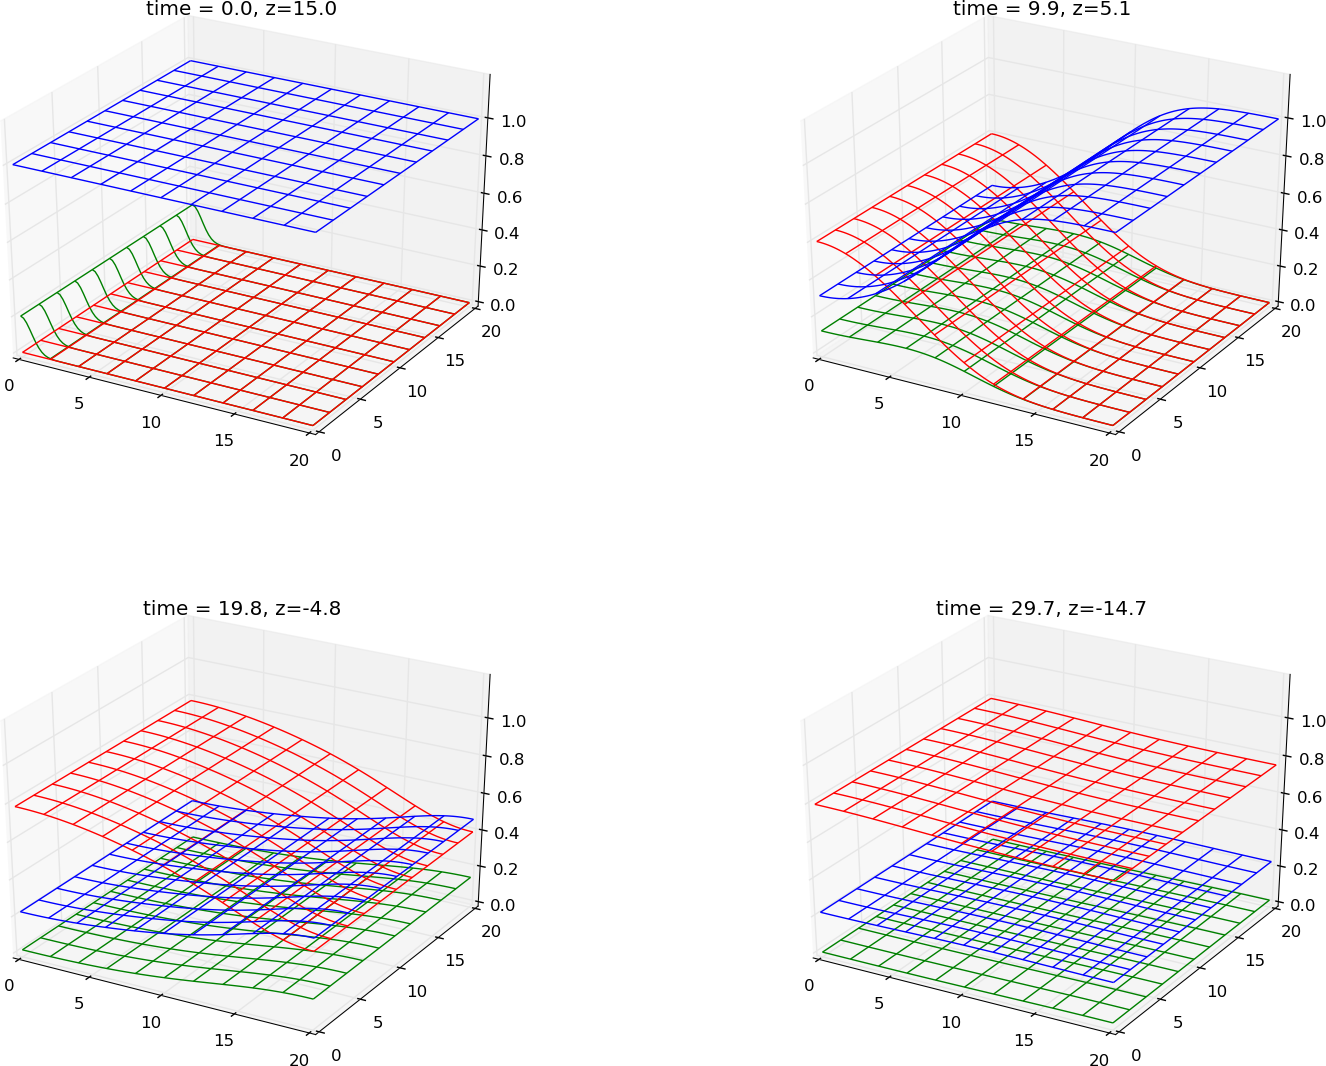
\includegraphics[width=0.8\linewidth]{plots/2D_gauss_sub.eps}}
  \caption{
  The PDE system (\ref{eq:simple_non_PDE}) simulated for a 2D system with $\lambda=0.5$. A gauss wave from $x=0$.
  }
\end{figure}
%\clearpage % flush figures 


\subsection{2D Gaussian function from x=0,y=0}


\begin{figure}[ht]
  \centerline{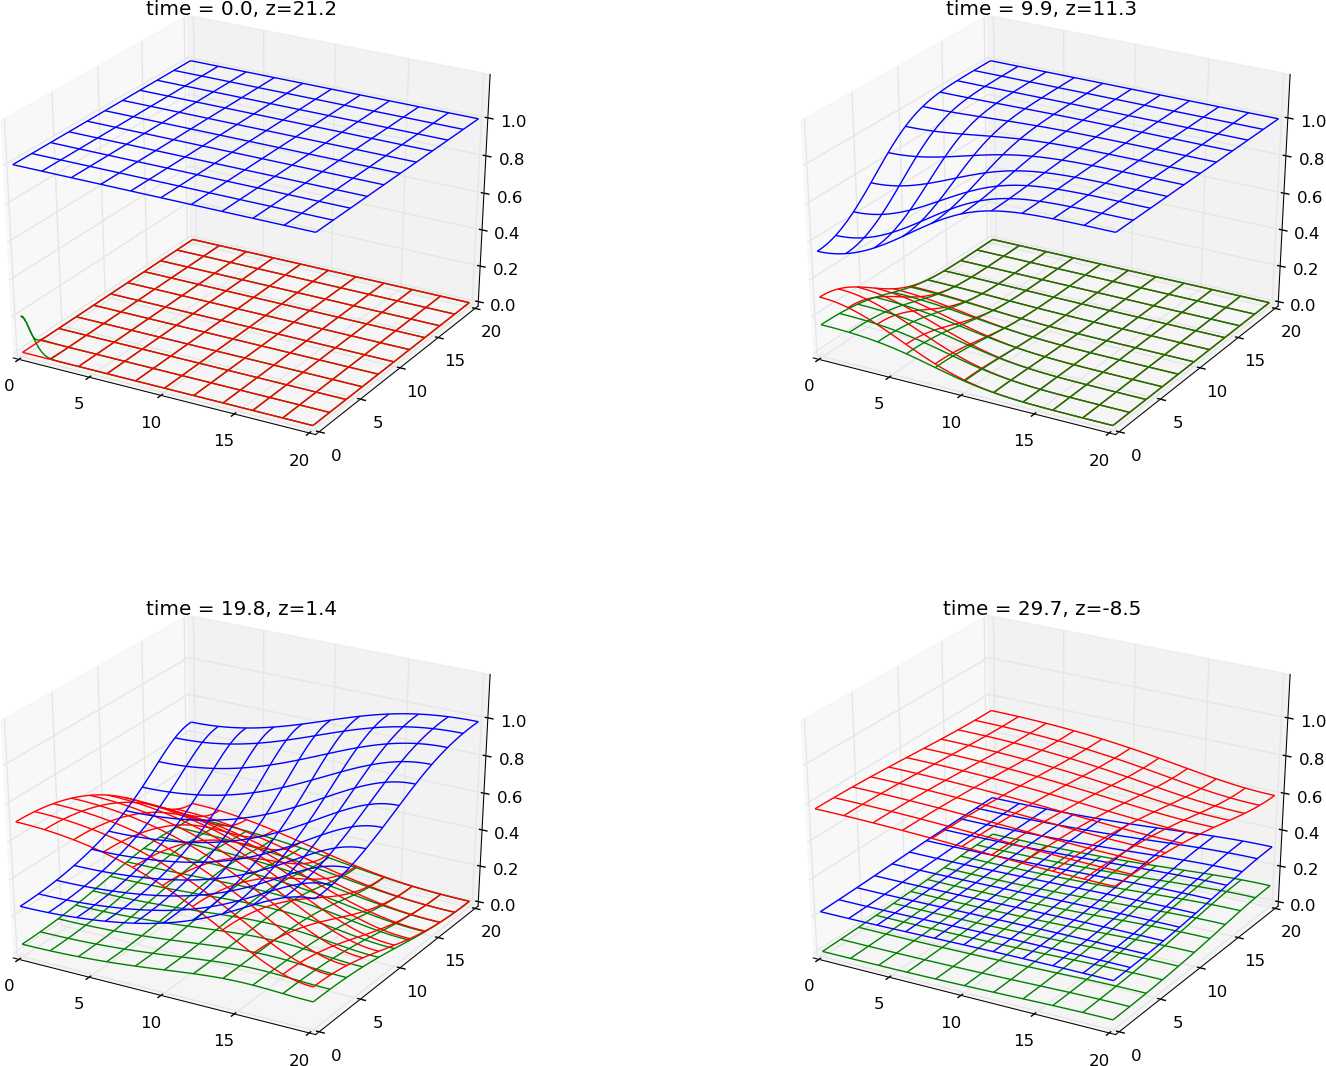
\includegraphics[width=0.8\linewidth]{plots/2D_gauss_one_sub.eps}}
  \caption{
  A gaussian function from $x=0,y=0$ based on the PDE system (\ref{eq:simple_non_PDE}) with $\lambda=0.5$
  }
\end{figure}
%\clearpage % flush figures 


\subsection{2D Gaussian function from x=0,y=0 with higher initial value}

\subsection{English Boarding School}


\begin{center}  % inline figure
  \centerline{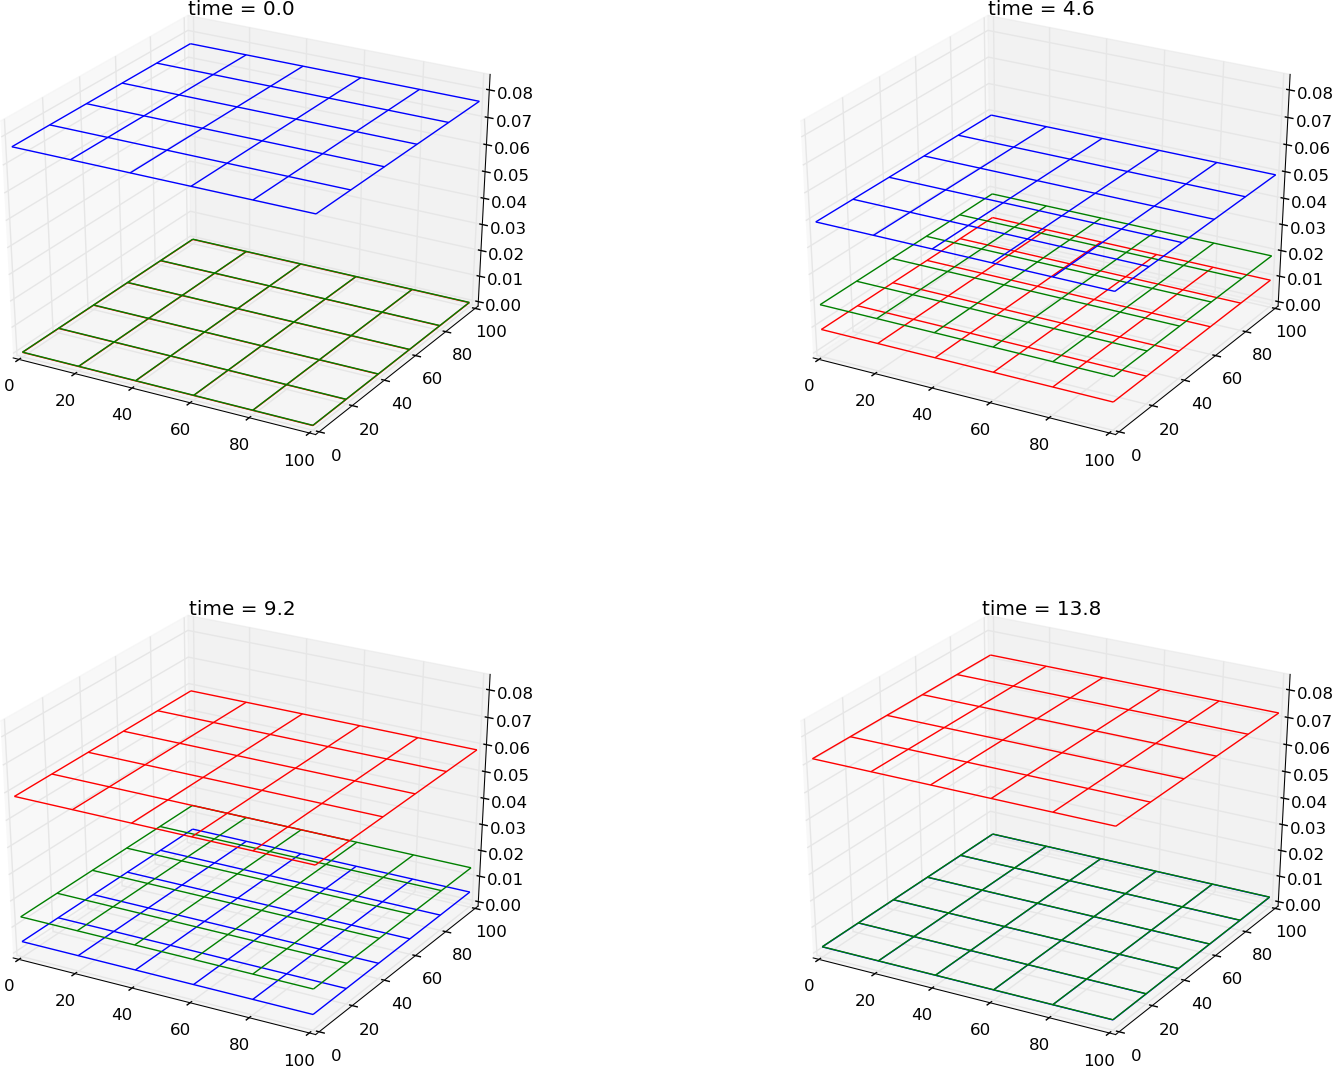
\includegraphics[width=0.8\linewidth]{plots/2D_british_school_sub.eps}}
\end{center}


\paragraph{Gaussian from the corner.}
\begin{center}  % inline figure
  \centerline{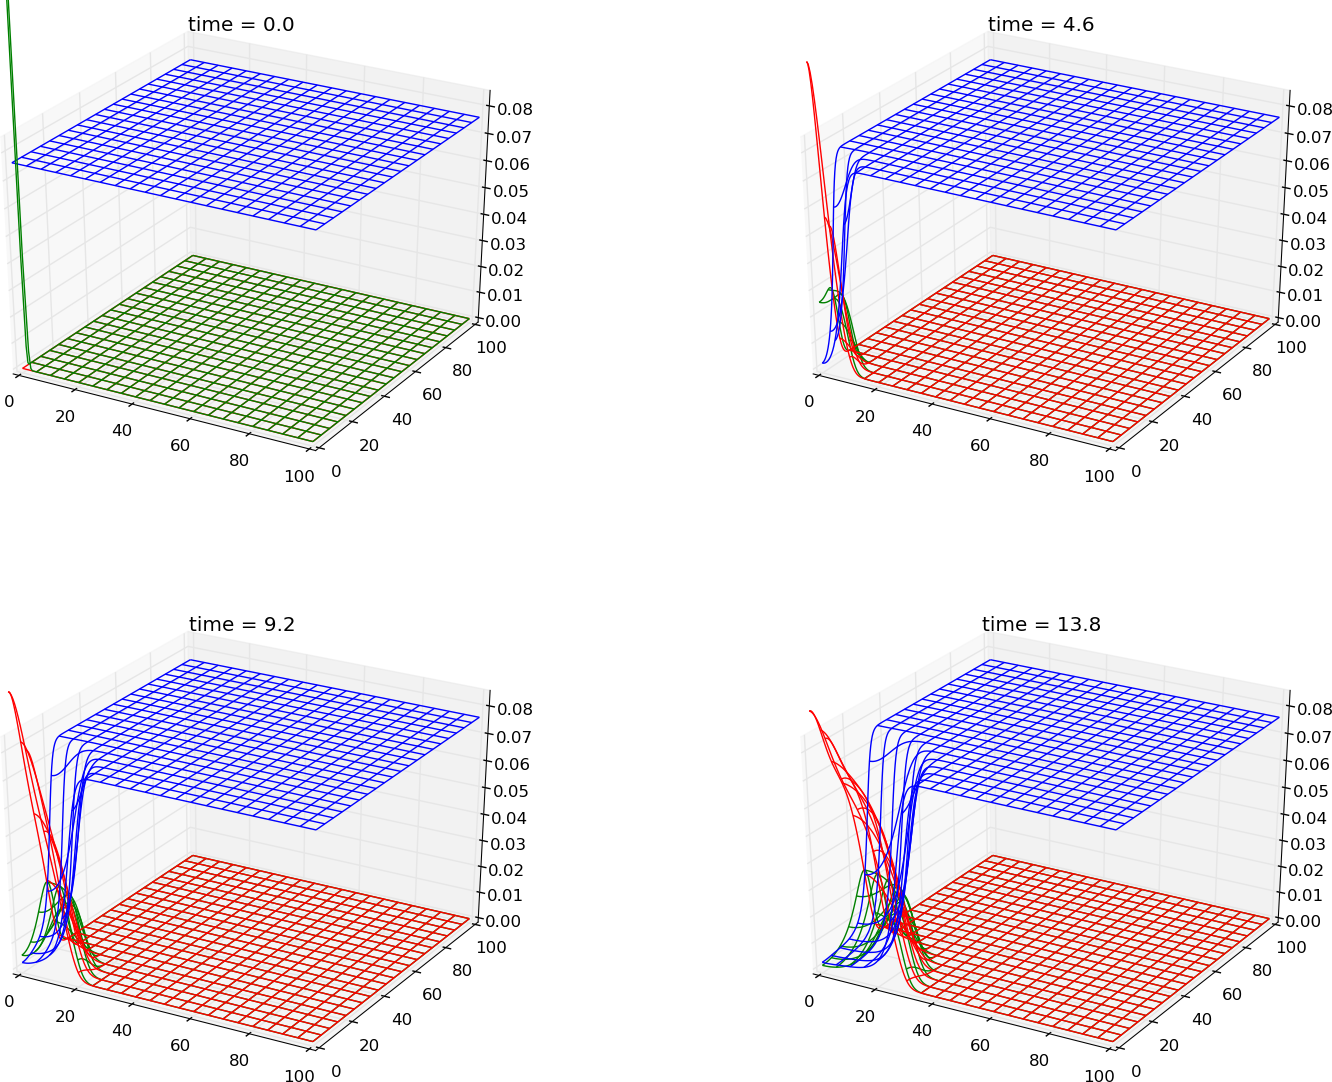
\includegraphics[width=0.8\linewidth]{plots/2D_british_school_gauss_corner_sub.eps}}
\end{center}


\paragraph{A long simulation on 100 Days.}
\begin{center}  % inline figure
  \centerline{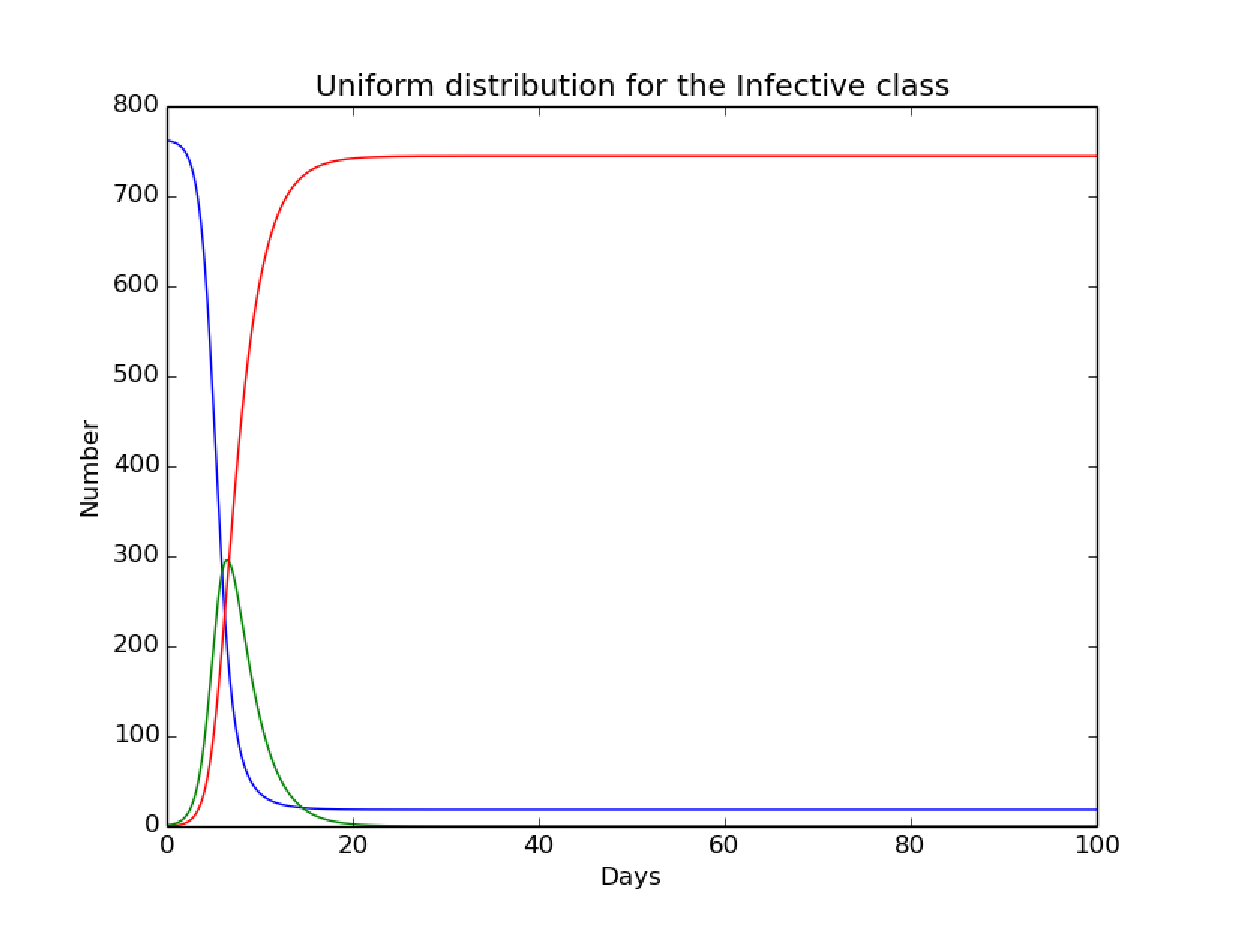
\includegraphics[width=0.8\linewidth]{plots/2D_british_school_long_number.eps}}
\end{center}



\begin{center}  % inline figure
  \centerline{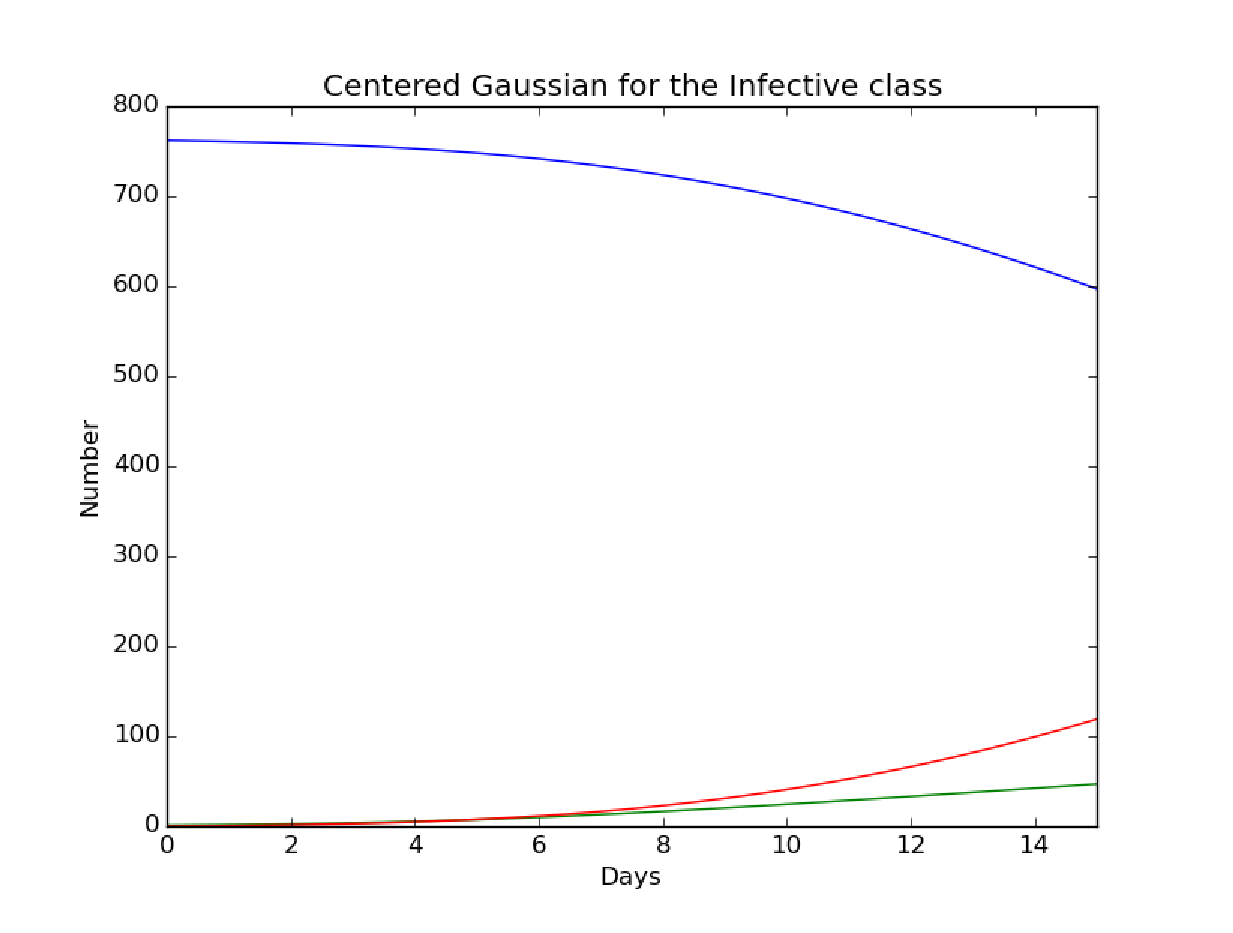
\includegraphics[width=0.8\linewidth]{plots/2D_british_school_gauss_long_number.eps}}
\end{center}



\begin{center}  % inline figure
  \centerline{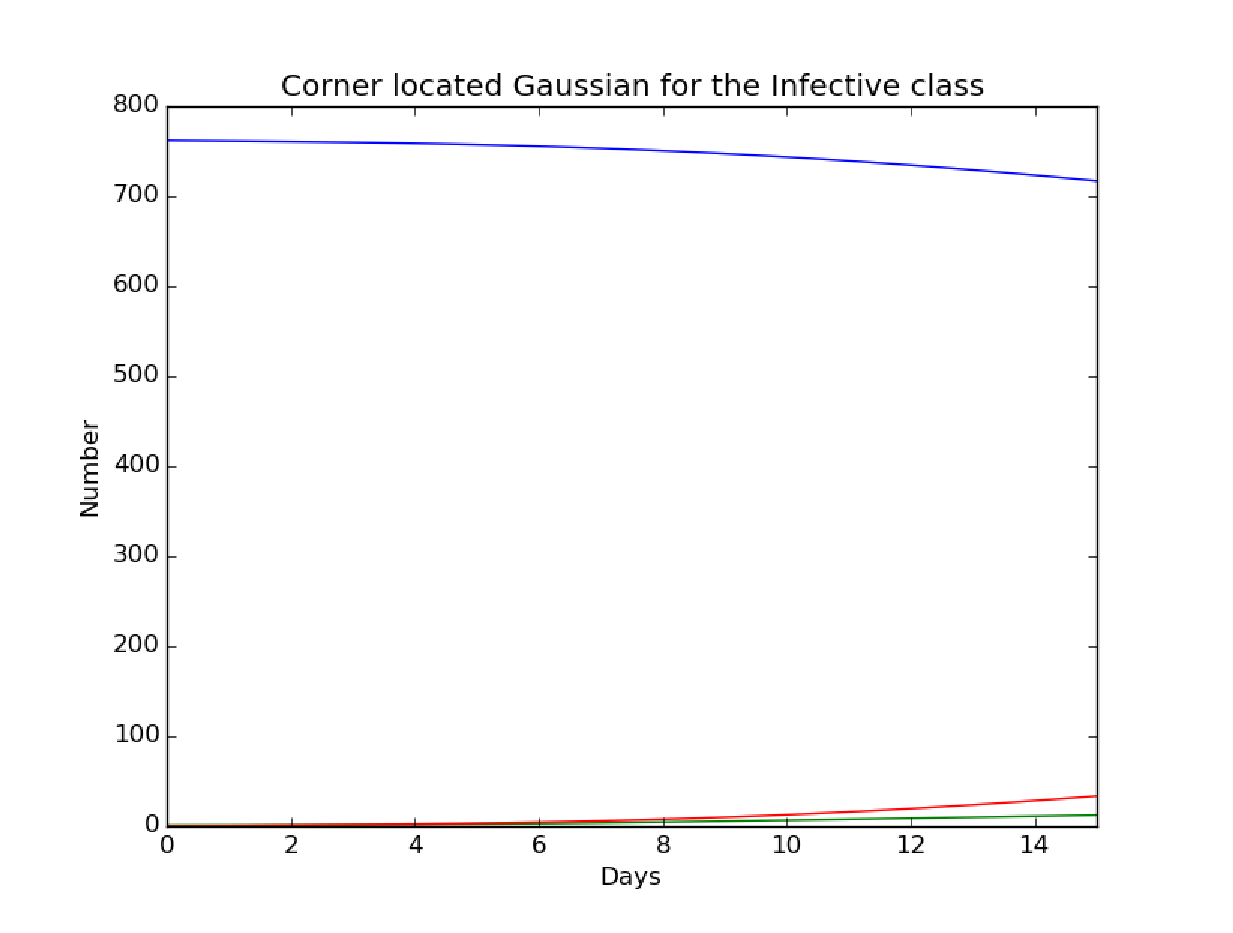
\includegraphics[width=0.8\linewidth]{plots/2D_british_school_gauss_corner_long_number.eps}}
\end{center}


\subsection{Zombiefication}
\paragraph{Verify the initial phase.}
\begin{center}  % inline figure
  \centerline{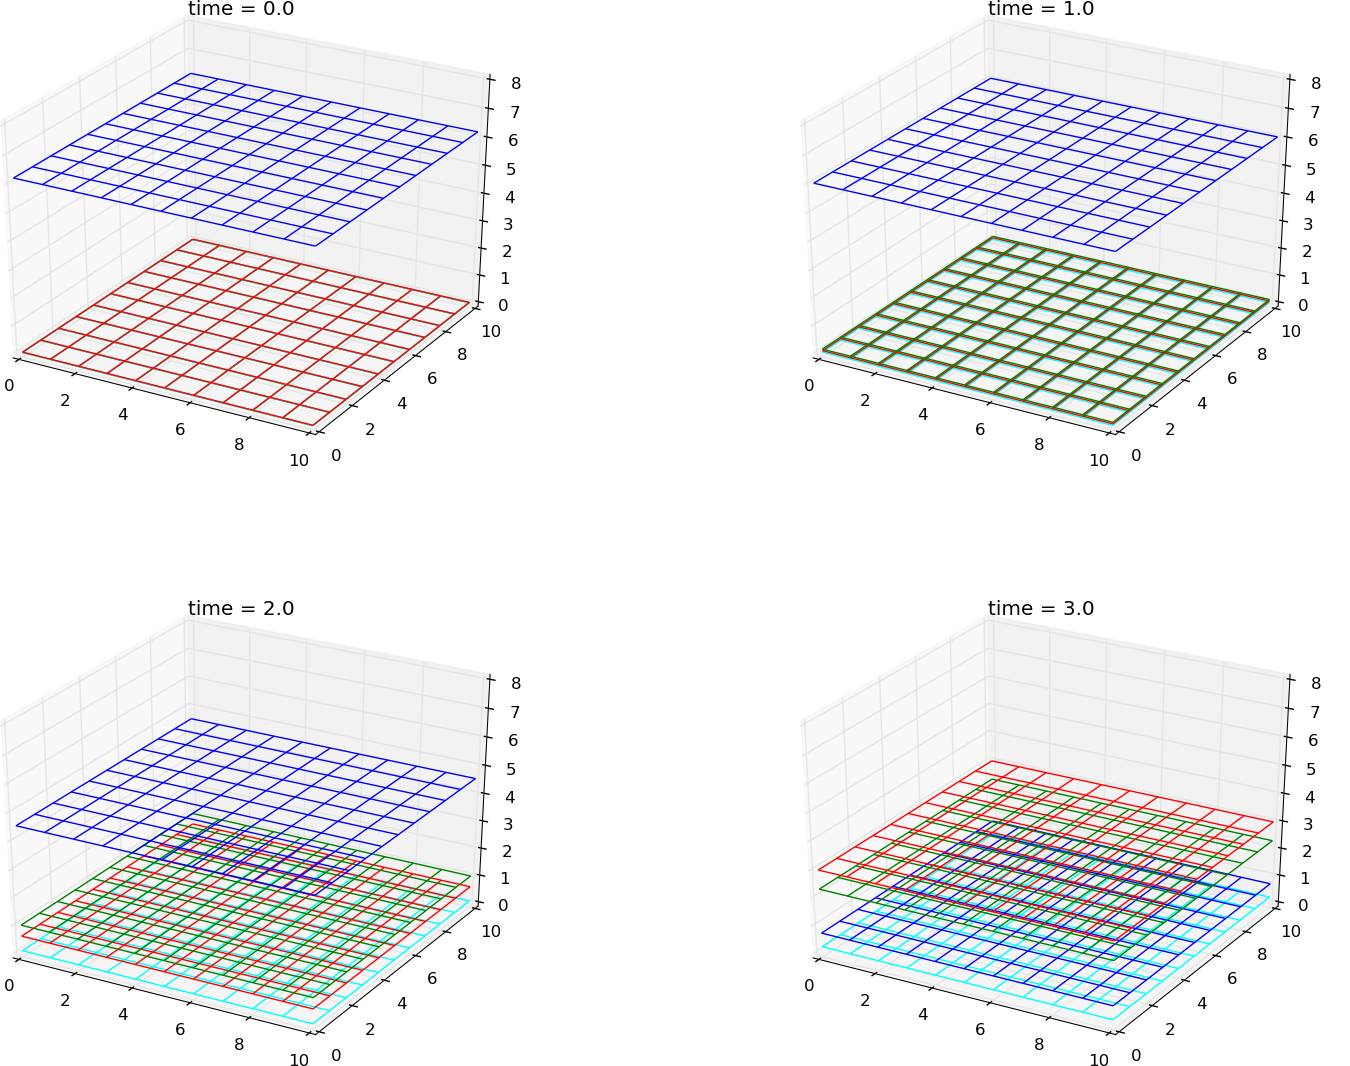
\includegraphics[width=0.8\linewidth]{plots/2D_zombie_initial_cond_sub.eps}}
\end{center}



\begin{figure}[ht]
  \centerline{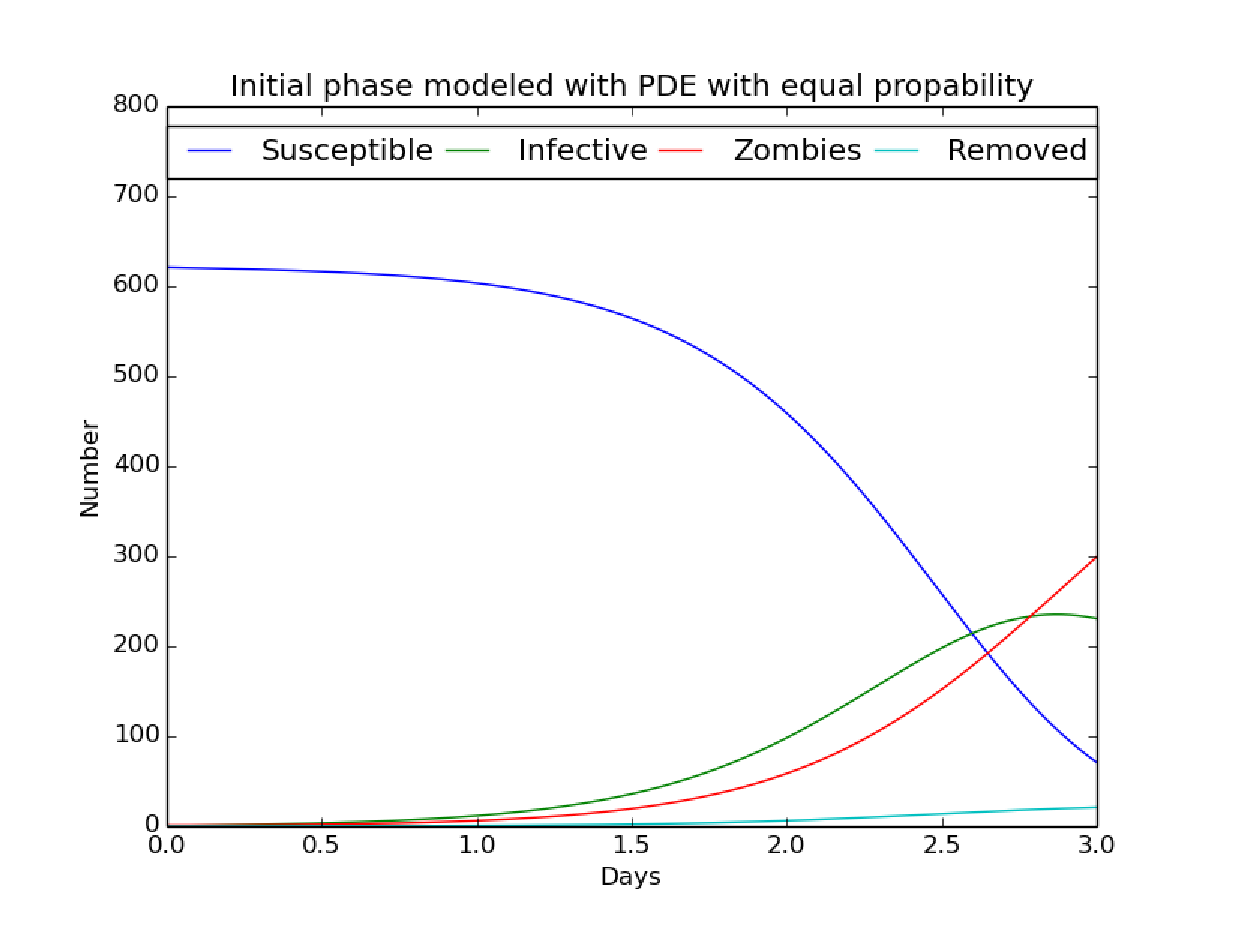
\includegraphics[width=0.8\linewidth]{plots/2D_zombie_initial_cond_number.eps}}
  \caption{
  Creates the same results as for the ODE system
  }
\end{figure}
%\clearpage % flush figures 


\paragraph{Three phases.}
\begin{center}  % inline figure
  \centerline{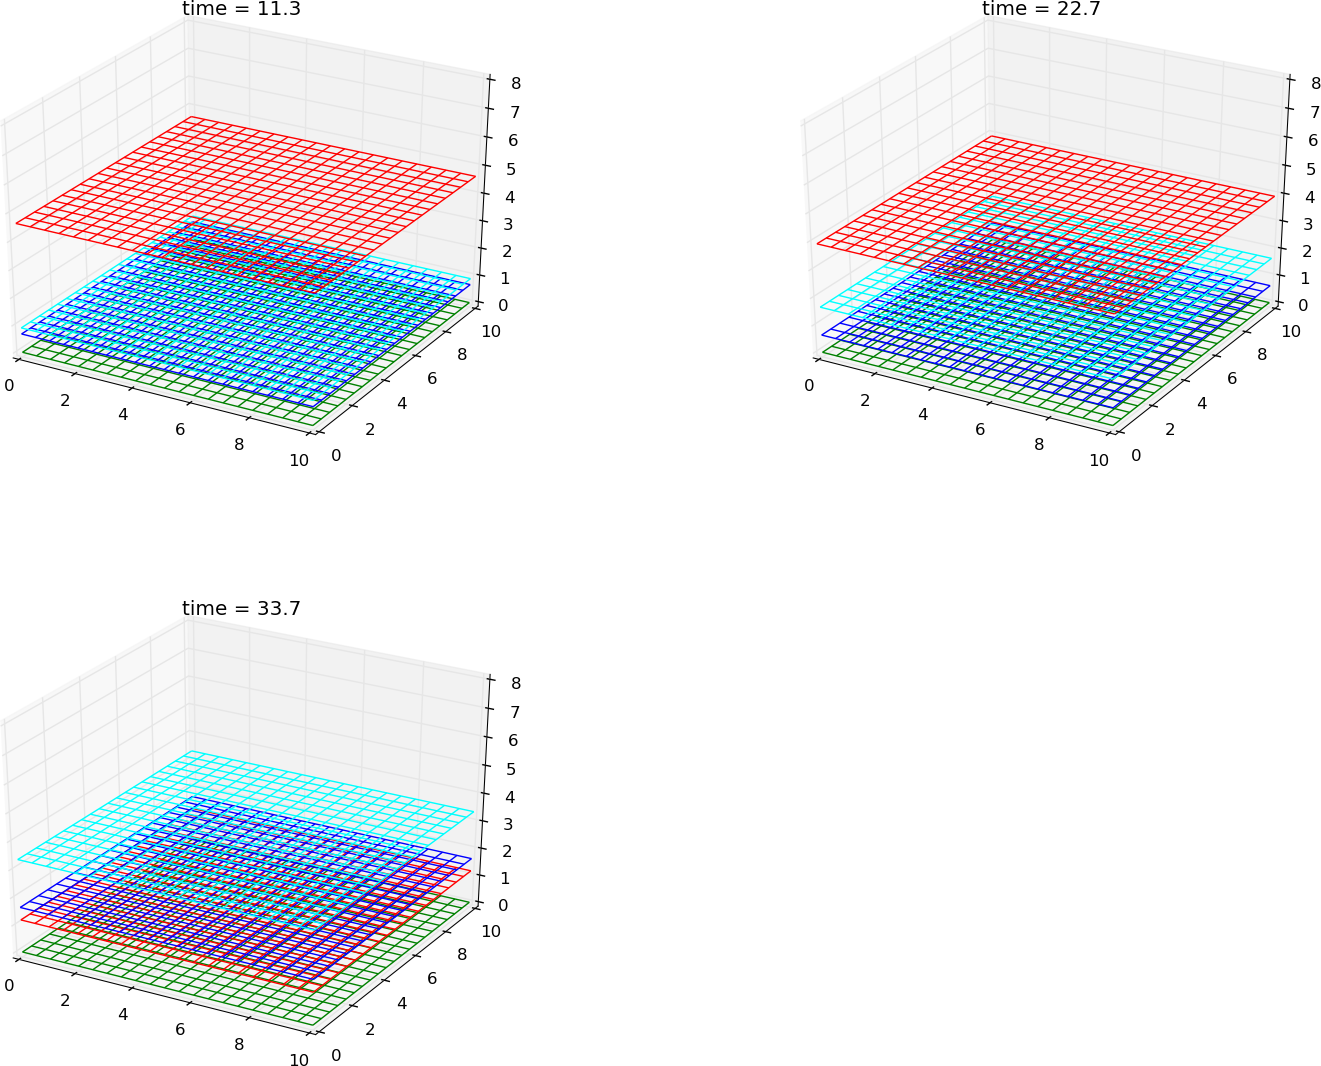
\includegraphics[width=0.8\linewidth]{plots/2D_zombie_three_phases_sub.eps}}
\end{center}


\paragraph{middle town.}
\begin{center}  % inline figure
  \centerline{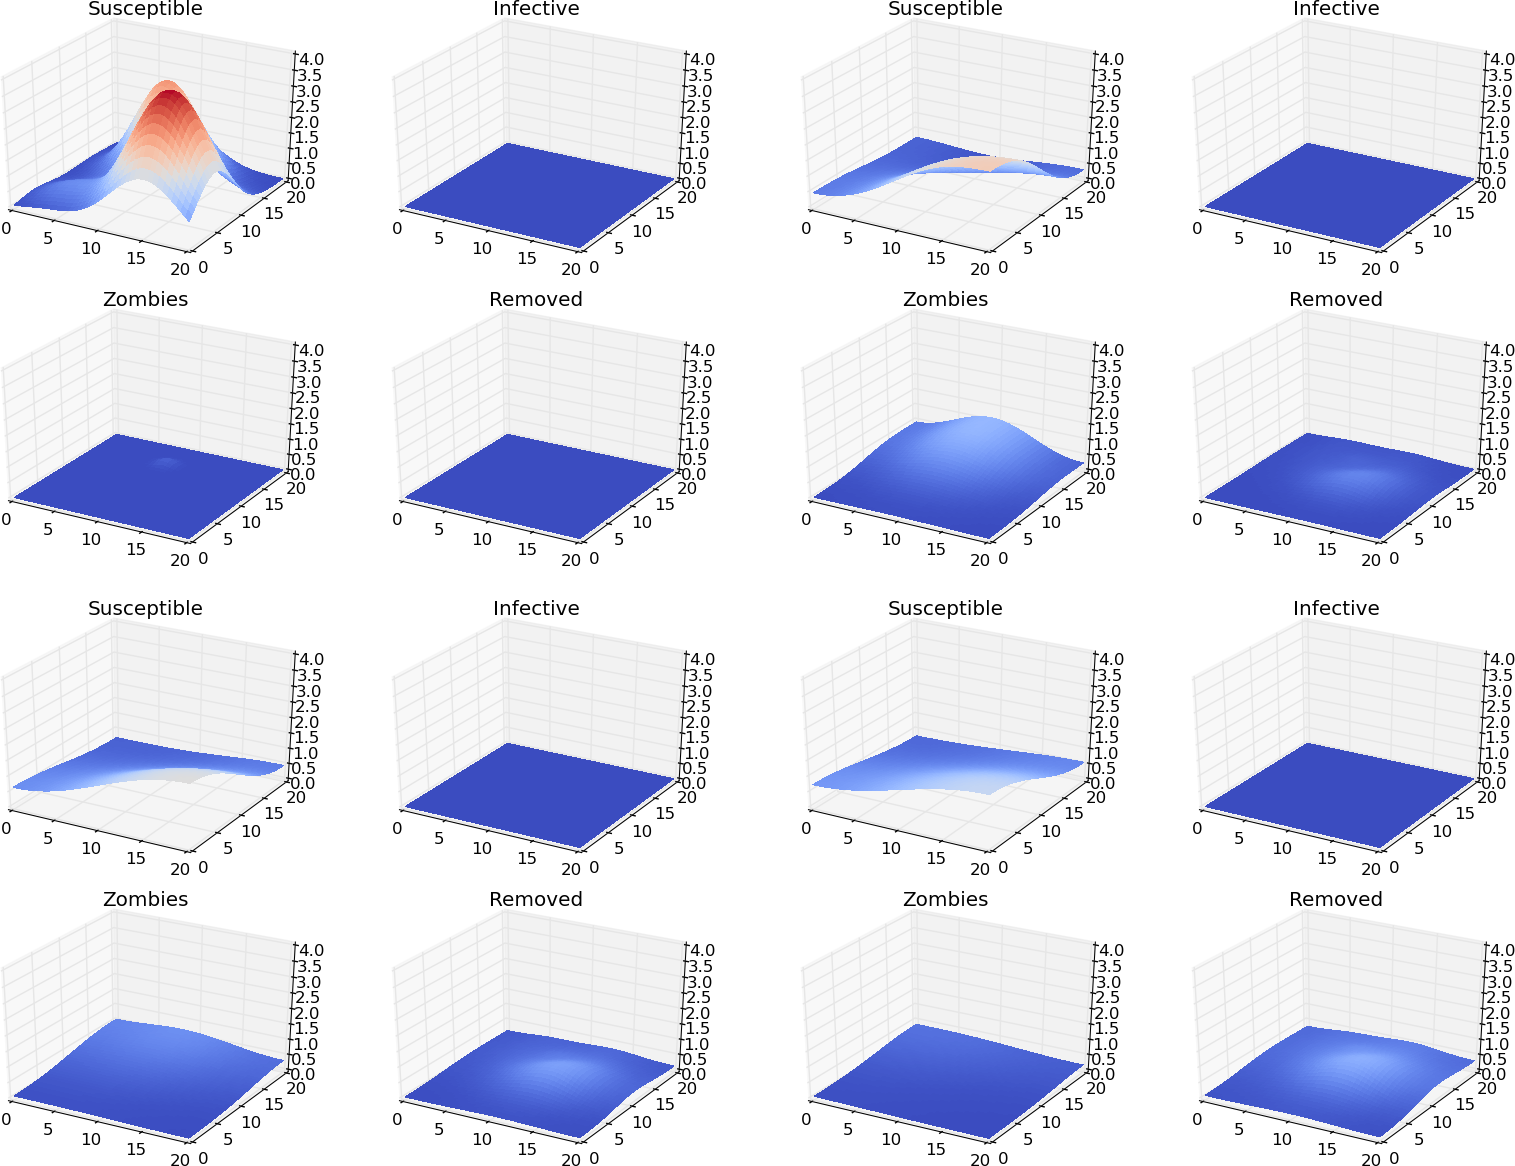
\includegraphics[width=0.8\linewidth]{plots/2D_zombie_three_phases_zombie_middle_town_surface_sub.eps}}
\end{center}


\paragraph{large town.}
\begin{center}  % inline figure
  \centerline{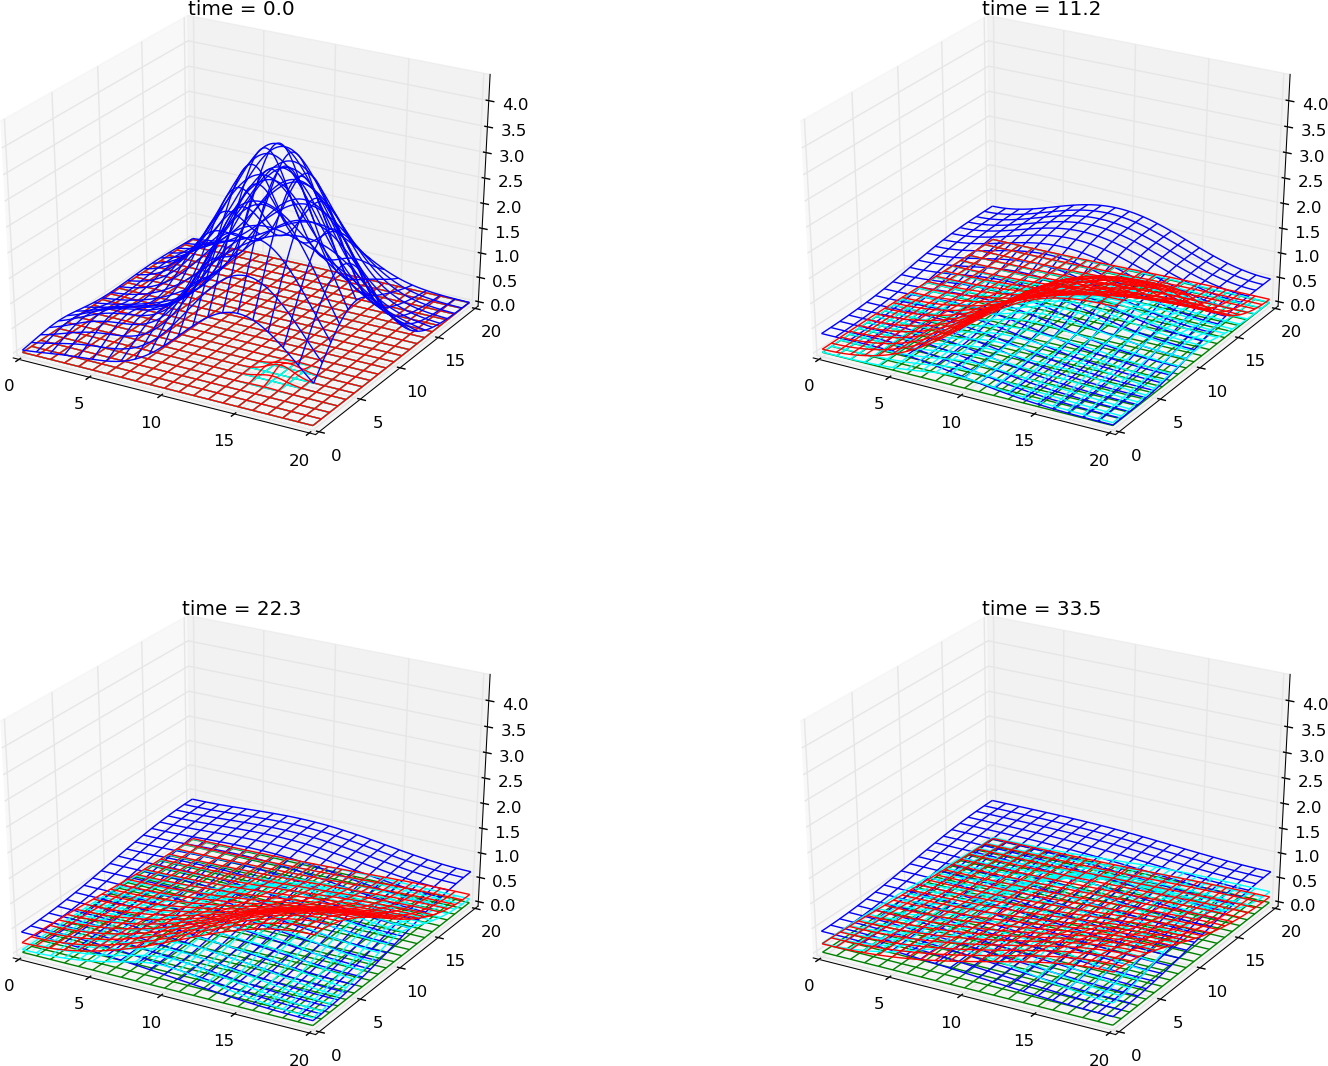
\includegraphics[width=0.8\linewidth]{plots/2D_zombie_three_phases_zombie_large_town_sub.eps}}
\end{center}


% MOVIE:[plots/2D_gaussian.webm, height=500 width=600] Travelling wave modeled with the same values as for 1D.
% MOVIE:[plots/2D_one_corner.webm, height=500 width=600] Starting the travelling wave from the corner.
% MOVIE:[plots/2D_initial_variable.webm, height=500 width=600] Travelling wave with a greater initial wave.
% MOVIE:[plots/2D_british_school.webm, height=500 width=600] Acts like the ODE system
% MOVIE:[plots/2D_british_school_gauss.webm, height=500 width=600] The sick one is placed in the center of the School area.
% MOVIE:[plots/2D_british_school_gauss_corner.webm, height=500 width=600] A wave of infected moves towards the school yard
% MOVIE:[plots/2D_zombie_initial_cond.webm, height=500 width=600]
% MOVIE:[plots/2D_zombie_three_phases.webm, height=500 width=600]
% MOVIE:[plots/2D_zombie_three_phases_zombie_small_town.webm, height=500 width=600] Created with different diffusion constants. The groups of susceptible are placed in three different areas.
% MOVIE:[plots/2D_zombie_three_phases_zombie_small_town_surface.webm, height=500 width=600] Created with different diffusion constants. The groups of susceptible are placed in three different areas.
% MOVIE:[plots/2D_zombie_three_phases_zombie_middle_town.webm, height=500 width=600] Created with different diffusion constants. The groups of susceptible are placed in three different areas.
% MOVIE:[plots/2D_zombie_three_phases_zombie_middle_town_surface.webm, height=500 width=600] Created with different diffusion constants. The groups of susceptible are placed in three different areas.
% MOVIE:[plots/2D_zombie_three_phases_zombie_large_town.webm, height=500 width=600] Created with different diffusion constants. The groups of susceptible are placed in three different areas.
% MOVIE:[plots/2D_zombie_three_phases_zombie_large_town_surface.webm, height=500 width=600] Created with different diffusion constants. The groups of susceptible are placed in three different areas.
% MOVIE:[plots/2D_zombie_three_phases_blindern_area_contourf.webm, height=500 width=600] Created with different diffusion constants. The groups of susceptible are placed in three different areas.
% MOVIE:[plots/2D_zombie_three_phases_blindern_area_3_ph_contourf.webm, height=500 width=600] Created with different diffusion constants. The groups of susceptible are placed in three different areas.



\bibliographystyle{plain}
\bibliography{../bibliography/papers}


% ------------------- end of main content ---------------


% #ifdef PREAMBLE
\printindex

\end{document}
% #endif

